\documentclass[12pt,a4paper,fleqn, onesside]{report}
%
\usepackage[T1]{fontenc}
\usepackage{amsmath, amssymb, amsthm}
\usepackage[danish,english]{babel}

\usepackage[ansinew]{inputenc}
%\usepackage[utf8]{inputenc} %Der skal anvendes utf8
\usepackage{epsfig}
\usepackage{graphicx}
\usepackage[]{mcode}
\usepackage{lmodern}
\usepackage{float}
\usepackage{setspace}
\usepackage{lscape}
\usepackage{hyperref}
\usepackage{cleveref}
\crefname{equation}{}{equations}
\crefname{figure}{figure}{figures}
\usepackage{tabu}
\usepackage{graphicx}
\usepackage{caption}
\usepackage{multirow}
\usepackage{spverbatim}
\usepackage{dirtytalk}
\usepackage{gensymb}
\usepackage{pdfpages}
\usepackage{mathpazo}
\usepackage{algpseudocode}
\usepackage{bm}
%\usepackage{subfig}
\usepackage{subfigure}
%\usepackage{mathptmx}
\onehalfspacing

\usepackage[top=25mm, left=30mm, right=30mm,bottom=25mm,headsep=10mm, footskip=12mm]{geometry}
%
\usepackage{fancyhdr}
\pagestyle{fancyplain}
\lhead[\thepage]{}

\begin{document}

% PAGE DE TITRE
\begin{titlepage}
\begin{center}
\vspace{4cm}
\Huge{\sc 30330 Image Analysis with Microcomputer}\\
\vspace{0.8cm}
\large{\sc Project report\\}
\vspace{1.2cm}
%\Huge {\sc Exam Report}\\
%\vspace{2cm}
\normalsize{by}\\
\vspace{1.2cm}
{\sc
\large Katleen Blanchet s150798  \\ 
Titouan Boulmier s150810\\
}
%\o{}
\vspace{2cm}
\begin{center}

\includegraphics[scale=2.2]{dtulogo2.jpg}
\end{center} 
\vspace{3.1cm}
\normalsize{\today}\\
\vspace{1.37cm}
\includegraphics[scale=0.7]{dtulogo.jpg}\\
\vspace{0.2cm}
\normalsize{Technical University of Denmark \\ Department of Electrical Engineering \\
}
\end{center}
\end{titlepage}
%\newpage
\thispagestyle{empty}
\selectlanguage{english}

\pagebreak
\pagenumbering{Roman}
\setcounter{page}{1}
\setcounter{tocdepth}{4}
\setcounter{secnumdepth}{4} 
\def\chaptername{Part}

% SOMMAIRE
\tableofcontents
\newpage
\pagenumbering{arabic}

% Intro
\section*{Introduction}
\addcontentsline{toc}{part}{Introduction}
The research of habitable planet is one of the major concerns of human beings. Indeed, this discovery, in addition to give hope of locating another species, would bring solutions to overpopulation. According to scientists, the main criterion for life is water. Since the properties of celestial bodies are disparate, a habitable zone was defined, considering that water can only exist at a specific range of temperature. If the temperature of the planet is too low, the water will freeze and conversely, it will evaporate if the temperature is too warm. The habitable zone is not fixed; it moves with the evolution of the sun. Mars is thought to have belonged to the zone once, due to its most hospitable climate after Earth. For a matter of fact, NASA's Mars Reconnaissance Orbiter has recently provided a strong evidence of water currently flowing on the Red Planet. It may then be possible to live on Mars and that is the aim of Mars one project: send a colony over there. The terraforming, which would change characteristics of Mars to make it suitable for humans, is also worth considering before colonization. In order to do so, scientists need to learn more about the features of the planet. Orbiters and rovers are already scanning mars surface and soil. Nevertheless, they lack the depth information, only equipped of Two Dimensional (2D) cameras. Their three dimensional (3D) scans have permitted to acquire it and to print a Martian meteorite on Earth in 2014. This information is useful for a better understanding of the rocks properties but that is not enough. Some missing data have delayed the 3D print. It could be interesting to provide to scientists a real time 3D map of a selected rock. It would be easier to study stones but the map could also help the robot to stabilize. With wind and an uneven ground, the rover is liable to move. The pattern recognition of a rock would be more robust by adding a 3D map. Samples could be collected being sure that the robot has taken the right piece. 

Furthermore, the 3D map could have several other applications. The features of the Martian soil acquired by the orbiting satellites are not exhaustive and lack of accuracy. Thus, applied to the area in front of the robot, the 3D map could detect new obstacles and update in real time the available map to distinguish modifications of the ground. It could also permit spacecrafts to determine a flat area to land in real time by analyzing the surface of the planet from space and during the descent. Moreover, the 3D map has other applications in completely different fields. Indeed, this technical can found, as example, in video games with environment recordings for real time augmented reality gaming, in medicine with skin surface measurement or skin roughness measurement, in cosmetic with wrinkle measurement and also in industry with 3D-automated optical inspection, volume measurement or Classification of grinding materials and tools.

However, the 3D mapping is not much used and is still improving. In this context, designing a system capable of carrying out a 3D map of a Martian rock would be profitable for future research. This is the purpose of this project, undertaken during the Image Analysis with Microcomputer course, under the supervision of Alessandro Massaro. Combining image and scene analysis, programming and robotics seems relevant for learning to work as an engineer.

This report is intended to our fellow students. The first part will bring additional knowledge required to understand the next developments. The design of the system is described in the next section, followed by its verification. To end, future work is addressed.

\chapter{Problem formulation and delimitation}
\section{Problem formulation}
\begin{figure}[H]
  \centering
  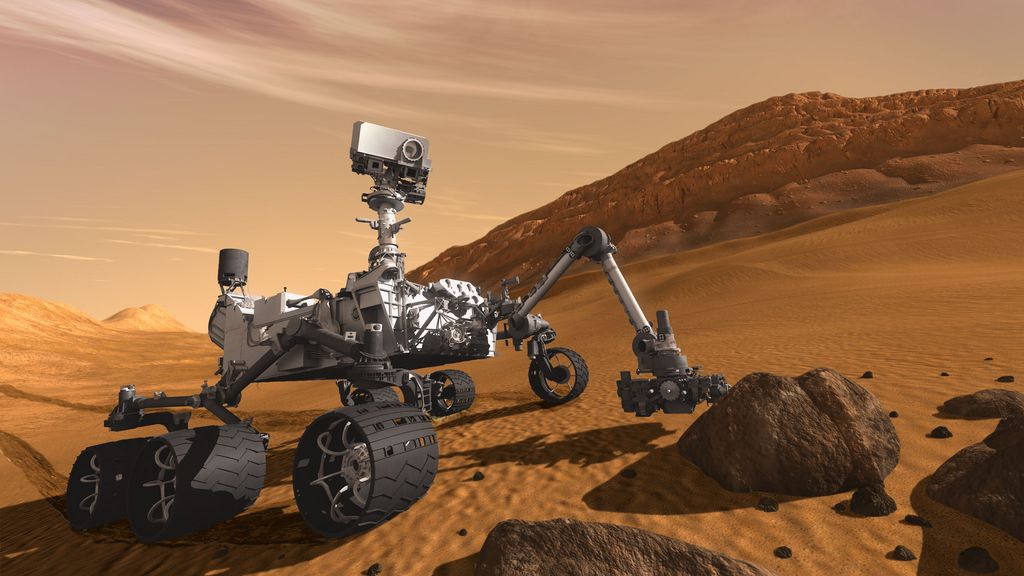
\includegraphics[scale=0.5]{fig/marsRover.jpg}
  \caption{Curiosity Rover with an embedded camera on a arm \cite{nasa}}
  \label{fig:CuriosityRover}
\end{figure}

In this report, we assume that we would like to send a rover on Mars, capable of communicating with Earth. Self-powered by solar panels, it will land at latitude 50� where it could get enough sunlight to recharge its lithium batteries. It is provided with an arm whose hand is replaced with a camera (see figure \ref{fig:CuriosityRover}). The latter will be used by scientists to observe relevant rocks to study. In order to accomplish this mission, once a stone is designed, the camera must be able to keep it in focus, despite the wind, the movement of the robot or any other perturbation. This implies a real time image analysis to be able to rectify the position of the camera. As a robust method is needed to maintain the stone in front of the arm, the correspondence problem is achieved by carrying out a 3D map of the surface. A luminous source should then be added to the rover to be projected on the surface containing the rock and detected by the camera.

This luminous source must be powerful enough to outshine the sunlight during the day, notwithstanding that the energy needed to make it work has to be negligible compared to the amount provided to the rover. Moreover, the characteristics of the camera need to be perfectly adapted to Mars, as once the rover has landed on the red planet, it would be impossible to adjust it. 

Will it be feasible to design such an embedded system, composed of a camera, a luminous source and algorithms, capable of keeping a rock in focus thanks to a 3D map, for an application on Mars soil? 


\section{Problem delimitation}
In order to design the rover's camera which will be used to study rocks and to implement a robust algorithm to carry out a 3D map of the rock's surface, different characteristics of Mars and of the target need to be specified. However, as all of them cannot be taken into account, some simplifications and choices will be assumed.

\paragraph*{Mars delimitation}
~\\
Plenty of missions on Mars have been realized and a great deal of data has already been gathered. Nevertheless, even if some of them will be used to designed our system, others will be simplified or even ignored.
The first simplification concern the atmosphere of Mars. Indeed, even if its composition is now well know, it will be assumed that the dirt on the surface Mars plus the different layers of the atmosphere absorb, or scatter, 10\% of the solar energy. Moreover, the influence on the image acquisition that the dirt between the target and the camera could have will not be taken into account.
The second reduction cover the temperature. Indeed, even if it can reach -143\textdegree C during winter, 27\textdegree C during summer and have around 60\textdegree C variations between daytime and nighttime\cite{wiki:temperature}, we will assume that the CCD sensor works well all the time.

\paragraph*{Target delimitation}
~\\
Regarding the target, that is to say the part of the rock being studied, it is supposed to :
\begin{itemize}
\item be vertical;
\item not exceed 2*2 meters
\item have an area between 0.1 and 1 square meters;
\item have a relief less than  meters.
\end{itemize}

\paragraph*{Camera delimitation}
~\\
Then, regarding the camera which is designed during this study, it is presumed to :
\begin{itemize}
\item be between one and two meters far from the target;
\item be right in front of the target, that is to say that the angle between the normal of the target's surface and the focal axis of the camera is 0\textdegree;
\item be able to capture the image of a target of 2 meters height maximum.
\end{itemize}

The different characteristics of target and the camera are represented figure \ref{fig:schema system}


\begin{figure}[h]
  %\centering
  \centerline{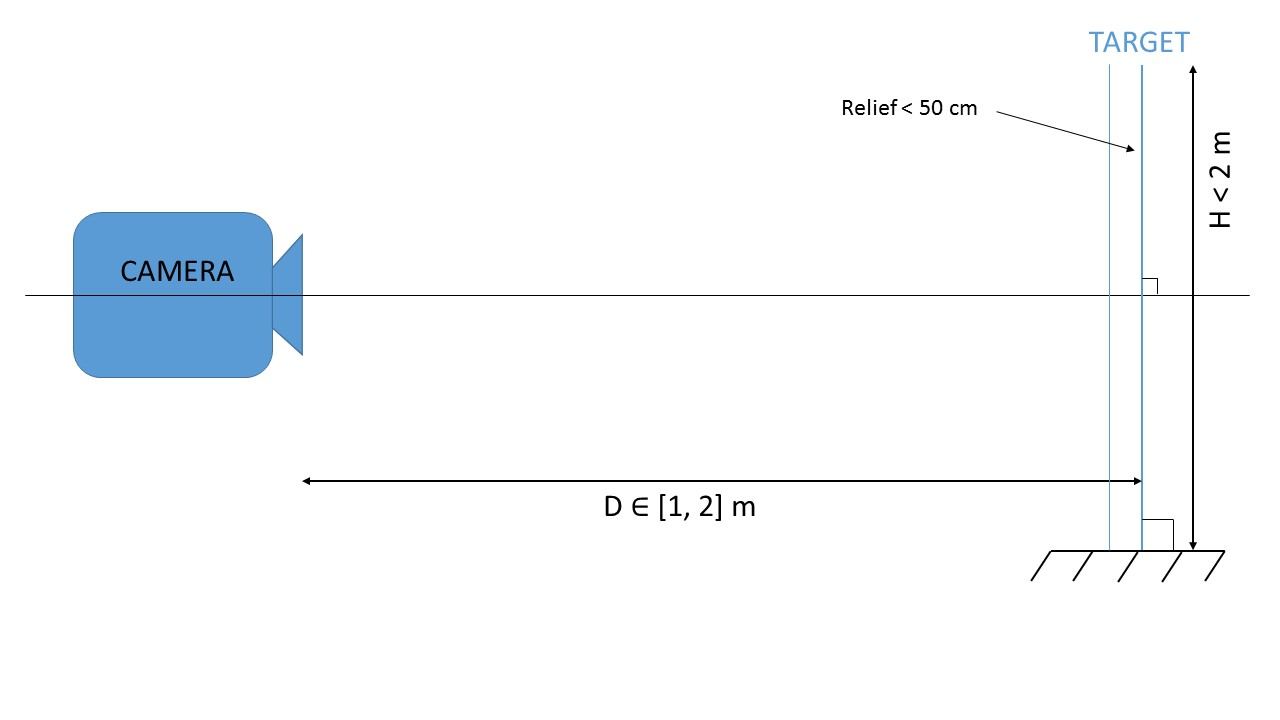
\includegraphics[scale=0.4]{fig/schemaSystem.jpg}}
  \caption{Schema of the scene}
  \label{fig:schema system}
\end{figure}



\chapter{Theory Section}
\section{Mars Features}
Mars, the fourth planet from the Sun (1.3814 to 1.6660 AU) is the second smallest planet of the the Solar System (its radius is 3389.5 km). Known as the ``Red Planet'' because of the amount of iron oxide on its surface, it has an orbital period of 668.6 sols (Mars' solar day), that is to say 687 days, with an average day length of 24h37m.
\subsection{Atmosphere of Mars}
Because of its thin atmosphere, Mars has surface features which present analogies with both Moon, through the impact craters, and Earth, with volcanoes, deserts, polar ice caps. It is mainly composed of carbon dioxide $CO_2$ (96,0 \% $\pm$ 0,7 \%), argon $Ar$ (1,93 \% $\pm$ 0,01 \%) and oxygen
$O_2$ (0,145 \% $\pm$ 0,009 \%). As the gravity of Mars is low, the height of the atmosphere is 11 km, more than one and a half times higher than the Earth's one (7 km). Moreover, due to this low gravity, the wind can disrupt a rover easier than on Earth and a large amount of suspended dust is perpetually present at the surface.

Regarding the dust, of which the particles have a mean diameter of $1,5 \micro m$, is continually injected into the atmosphere by wind or dust devils (a 12 km high one can be seen 12 Figure \ref{fig:poussiere}). Such eddies are far from anecdotal because they bring dust to significant volumes of the atmosphere. Even if the amount of dust is never very massive, it can be lifted by winds slower than 2 $m/s$ and maintained indefinitely by wind of only 0,8 $m/s$.

\begin{figure}[h]
  \centerline{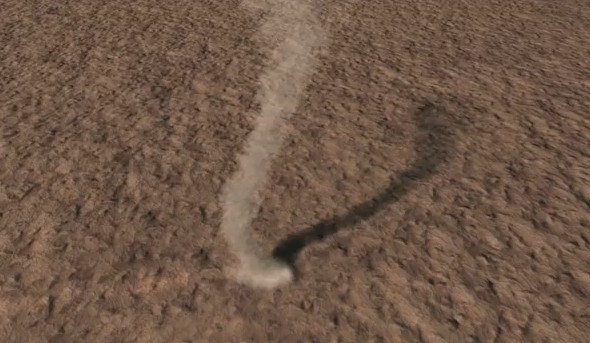
\includegraphics[scale=0.6]{fig/poussiere.jpg}}
  \caption{Dust Devil. Mars Reconnaissance Orbiter, made by HiRISE on Feb. 16, 2012}
  \label{fig:poussiere}
\end{figure}

Moreover, regarding the wind on Mars, in low altitudes, the Hadley circulation\footnote{movement on a planetary level of the layers of gases surrounding the planet} dominate and is almost the same process which, on Earth, generate the Trade winds. In high altitudes, a battery of areas of high and low pressure, named baroclinic pressure waves\footnote{In meteorology a baroclinic atmosphere is one for which the density depends on both the temperature and the pressure}, dominates the weather. The Mars wind lift a large amount of dust and can even trigger huge dust storms which can affect the while atmosphere (see Figure \ref{fig:storm}). Cyclonic storms can also appears on Mars. Indeed, cyclones similar to the ones of Earth tend to create during summer in the northern hemisphere but only in high latitudes.

\begin{figure}[h]
  \centerline{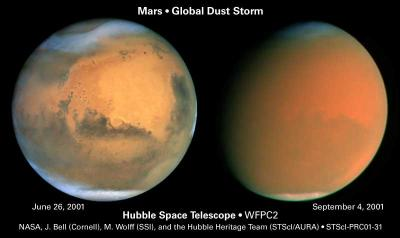
\includegraphics[scale=0.9]{fig/storm.jpg}}
  \caption{Two views of Mars with spatial telescope Hubble before and after the big dust storm in 2001}
  \label{fig:storm}
\end{figure}
\subsection{Climate of Mars}
\label{climate}
Because of its distance to the Sun bigger than the one of Earth, Mars receives less solar energy \ref{Irradiance}. Additionally, as its atmosphere is thinner, there is only a negligible greenhouse effect, and hence the average temperature is around -63\textdegree C on the surface of Mars with wide variations between daylight and night. \\
Then, the obliquity of Mars is close to the one of Earth (respectively 25,19\textdegree and 23,44\textdegree) but the eccentricity of Mars is bigger (0,09332 against 0,01671 for Earth) which means that, if Mars has similar seasons to Earth, they have different intensity and duration during the martian year. Thus, the northern hemisphere has seasons less pronounced than the southern hemisphere because its aphelion is at the end of spring and its perihelion at the end of autumn. Thus, there are short and soft winters and long and fresh summers in the northern hemisphere. On the opposite, the southern hemisphere has very pronounced seasons with long and cold winters and short and warmer summers than in the northern hemisphere. That is why there are higher temperature differences in the south.
\subsection{Albedo}
\label{albedo}
Mars surface is covered by sand and volcanic rocks. The first purpose of this project is to allow scientists to examine these rocks through the camera. To achieve it, it is needed to know their characteristics, especially their albedo. As a reminder, the albedo is the fraction of incident light which is reflected from a surface. We can assume that the power reflection of Martian rocks is the same than on Earth. Then, to cover a wild range of rocks, the albedos of a black and of a white stone would be considered. Charcoal, as a dark rock, is a powerful absorber of the sun radiation, with an albedo around 0.05. On the contrary, chalks are poor absorbers and their albedo reach 0.45 according to \cite{albedo}. In the following parts of the report, it will be taken for granted that Martian rocks have an albedo between 5 and 45\%.
\section{State of Art of the Depth Mapping}
Traditional cameras only take 2D pictures, with horizontal and vertical information. To reproduce the human vision useful in various applications such as the stabilization of a Martian rover arm in front of a rock to be analysed, it is often needed to add the depth data to get 3D coordinates of each pixel of the images. The depth mapping, also called 3D surface measurement or 3D imaging techniques etc, is carried out by two non-contact major methods as specified by \cite{sansoni2009state}: \say{projecting (in the active form) or acquiring (in the passive form) electromagnetic energy onto/from an object followed by recording the transmitted or reflected energy}. They can be divided into two categories, the non-optical and optical sensing. The first one generally uses acoustic and electromagnetic sensors to determine the distance from the system to the object, by assessing the duration of a round trip of a pulse. In the latter the light permits to get the depth. We will focus on this last technique as it will be more convenient to achieve it on Mars. Active optical sensing uses an additional light source where as passive optical sensing works only with the irradiance reaching the scene and the radiance of the object. 

\subsection{Principal Techniques Based on Image Analysis}
We will address only methods using image analysis as this is the purpose of the course.
Stereo vision and Photogrammetry systems are passive. The principle of the first is based on the utilisation of two or more cameras to record the scene. The reconstruction of the 3D is carried out by solving a correspondence problem with the identification of patterns in two or several images. The photogrammetry method calculates the depth by taking pictures from different points of view of a scene, through a camera preliminary calibrated. Both techniques demand a high computing power. Thus they are dismissed since the Rover cannot provide too much power to the embedded processor. 

In active optical sensing, laser triangulators and structured light can be distinguished. They share the same approach: a beam or a pattern is projected through a laser source towards the object and its position on the image acquired by the camera is measured. Then, the distance from the camera to the object (the depth) is found by applying a triangulation technique. The difference between the two methods is that it is needed to scan the whole object for the laser triangulators one. Indeed, only a beam or a laser strip reaches it at once. The experiment has to be repeated several times to have an exhaustive 3D map. Regarding the structured light approach, unique patterns are projected simultaneously which allows to obtain the depth data at once if the object is small but in any case, it reduces a lot the number of acquisitions compared to the laser triangulators. According to \cite{tuto}, the patterns can be in 3D but they are rare. 2D patterns are the most common and easier to implement. Depending on the scene motion, the structured light method can be classified into multi-shot and single-shot. If the scene is moving, the acquisition time must be short and thus, one picture should be enough to get the desired information. On the other hand, if no constraint is given, several pictures can be taken and a pattern adapted to sequential can be selected. In our case, the scene does not move but the robot arm could move and thus needs to be stabilized. That is why only single-shot structured light will be considered.

In the future part of the report, the implementation and experiments will be performed through laser triangulators techniques and structured light with a unicolor grid as a pattern. They are easier to set up but will only give us a partial depth map. To obtain a complete 3D map in a single shot, more complex patterns should be applied to the martian rock. Some methods that could be carried out then are described below. 
\subsection{M-array Pattern Projection Method \cite{morita1988reconstruction}}

The binary M-array pattern projection method consists in projecting dark and light dots. The color of each dot represents a 0 (dark) or 1 (light) of the M-array pattern. The spatial coordinates of each dot matched with a projected one of the pattern can be determined by triangulation. However, pattern disorders occur often in the observed pattern and some dots cannot be matched. One of the asset of this method is the detection and correction of pattern disorders.

\subsubsection{Pattern Disorders}
\label{PatternDisorders}
According to \cite{morita1988reconstruction}, there are three different types of pattern disorder.
\begin{itemize}
\item Deficiency of dots. If there are several objects in the scene, an object may obstruct the pattern. On the Figure \ref{fig:disorder1}, the first, second and third dots are not visible by the camera.
\item Displacement due to Difference in Depth : in comparison to the initial pattern projected, the dots may shift because of the depth of each object. On the Figure \ref{fig:disorder1}, the dots 4 to 6 on the object 2 have shifted to the left compared with the dots of object 1.
\item Permutation of dots : if an object is in front of another, the order of dots may change. On the Figure \ref{fig:disorder1}, the dot 3 has changed of order and is the fourth one from the point of view of the camera.
\end{itemize}

\begin{figure}[h]
  %\centering
  \centerline{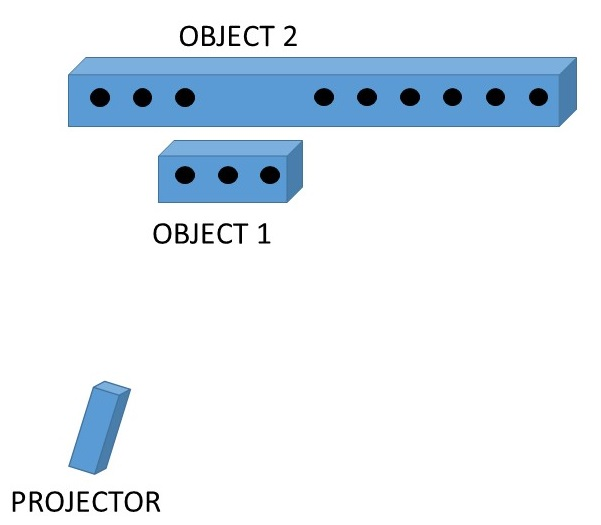
\includegraphics[scale=0.6]{fig/disorder1.jpg}}
  \caption{Pattern Disorders}
  \label{fig:disorder1}
\end{figure}






\subsubsection{Correction of Pattern Disorders}
There are four steps in the matching of the observed dots with those of the pattern and the correction of the pattern disorders.





\paragraph*{Temporary Array}
~~\\
The image recorded is analyzed line per line of dots and a 2-D array which contains the numbers of the observed dots is created. The array can be computed by these steps :
\begin{itemize}
\item Creation of the array (all the elements are set to zero).
\item Scan of the image to detect dots. Each time a dot is found, its value and position (center) are saved into 1-D arrays VALUE, X and Y.
\item The position of the dots are quantized using X and Y so that adjoining dots have consecutive quantized coordinates.
\item Insertion of the number of each dot into the array (the location into the array corresponds to the quantized coordinates).
\end{itemize}

This temporary array (T-array) may has some vacant places due to disorder pattern.

\paragraph*{Grow}
~~\\
Each element of the T-array gets an index (column number of the M-array). To do so, a window is defined and applied to the T-array and the M-array where the elements into the window of each array have the same value. The element into the window of the T-array can be indexed using the M-array and the two windows moved simultaneously by one column or row. This is repeated until a difference between the two windows is detected. New windows are then initialized elsewhere. The grow terminate when no window can be initialized to an area of the T-array where there is no index yet.


\paragraph*{Correction of Pattern Disorders}
~~\\
The detection step is is carried out during the growing and is explain below using an example. We use a 3$\times$4 window.
\begin{itemize}
\item step 1 : the region growing starts at (0',0') and (0,0) on the T-array and M-array (see Figure \ref{fig:detect} a).
\item step 2 : the window slides to the right until a difference between the two arrays is detected (see Figure \ref{fig:detect} b).
\item step 3 : In the T-array, the window is shifted to the right until the error is on the left side of the window. In the M-array, the window is moved until it matches with the one of the T-array (see Figure \ref{fig:detect} c).
\item step 4 : the windows now slides to the left and all the indices of the columns of the T-array are reset according to the two windows until another difference is detected.
\end{itemize}

\begin{figure}[h]
	\centering
	\hspace*{-2cm}
   \begin{minipage}[b]{0.50\linewidth}
      \centering 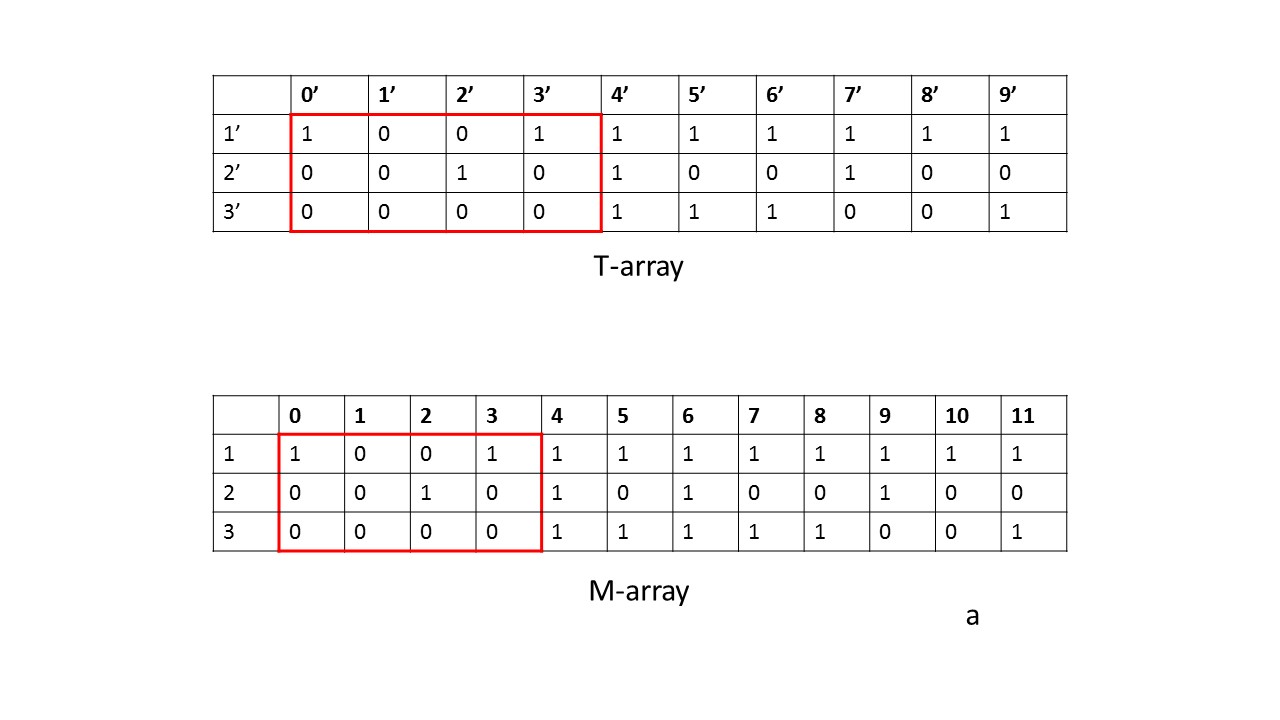
\includegraphics[scale=0.3]{fig/detect1.jpg}
      %\caption{\it Legend 1}
   \end{minipage}\hfill
   \begin{minipage}[b]{0.50\linewidth}   
      \centering 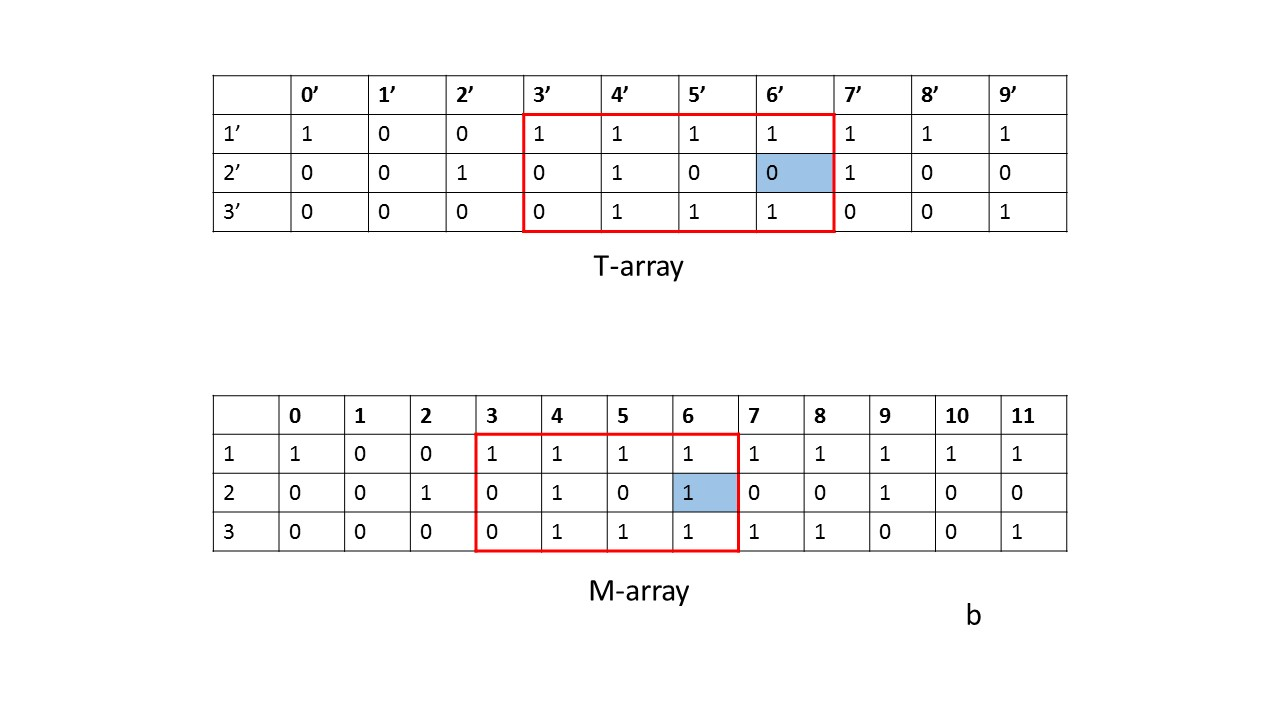
\includegraphics[scale=0.3]{fig/detect2.jpg}
      %\caption{Legend 2}
   \end{minipage}
	\hspace*{-2cm}
   \begin{minipage}[b]{0.50\linewidth}
      \centering 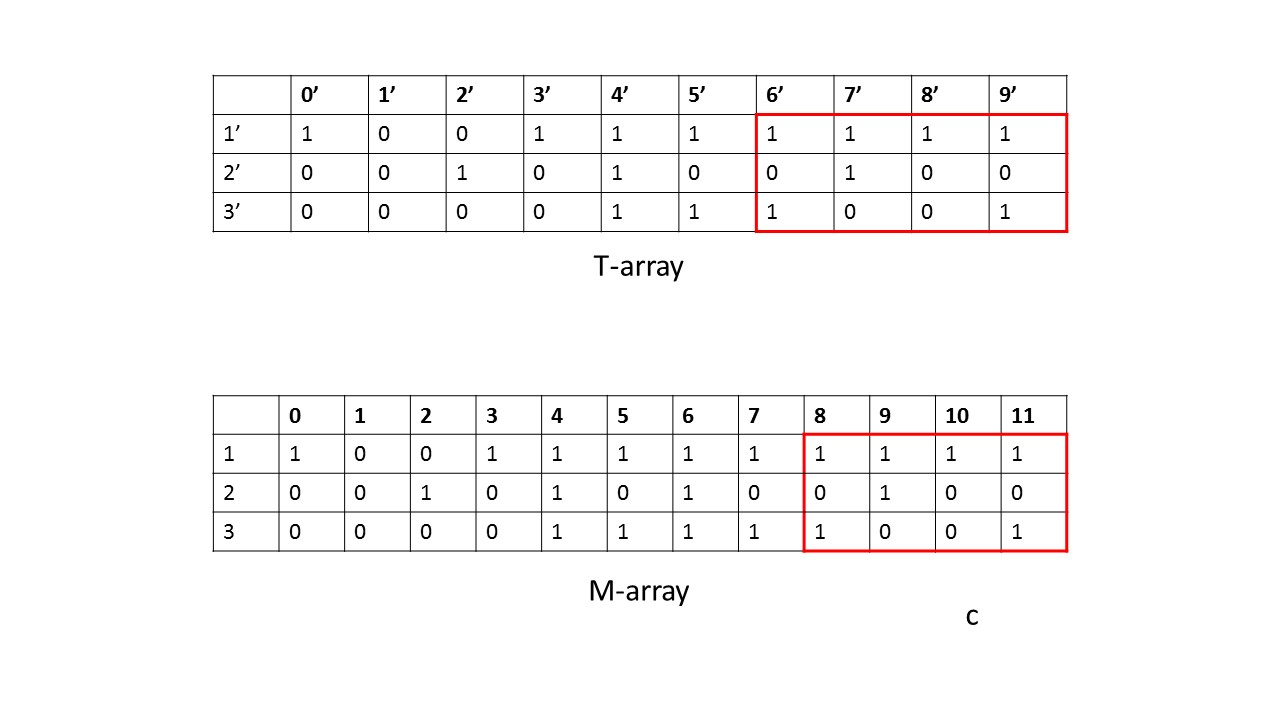
\includegraphics[scale=0.3]{fig/detect3.jpg}
      %\caption{Legend 3}
   \end{minipage}\hfill
   \begin{minipage}[b]{0.50\linewidth}   
      \centering 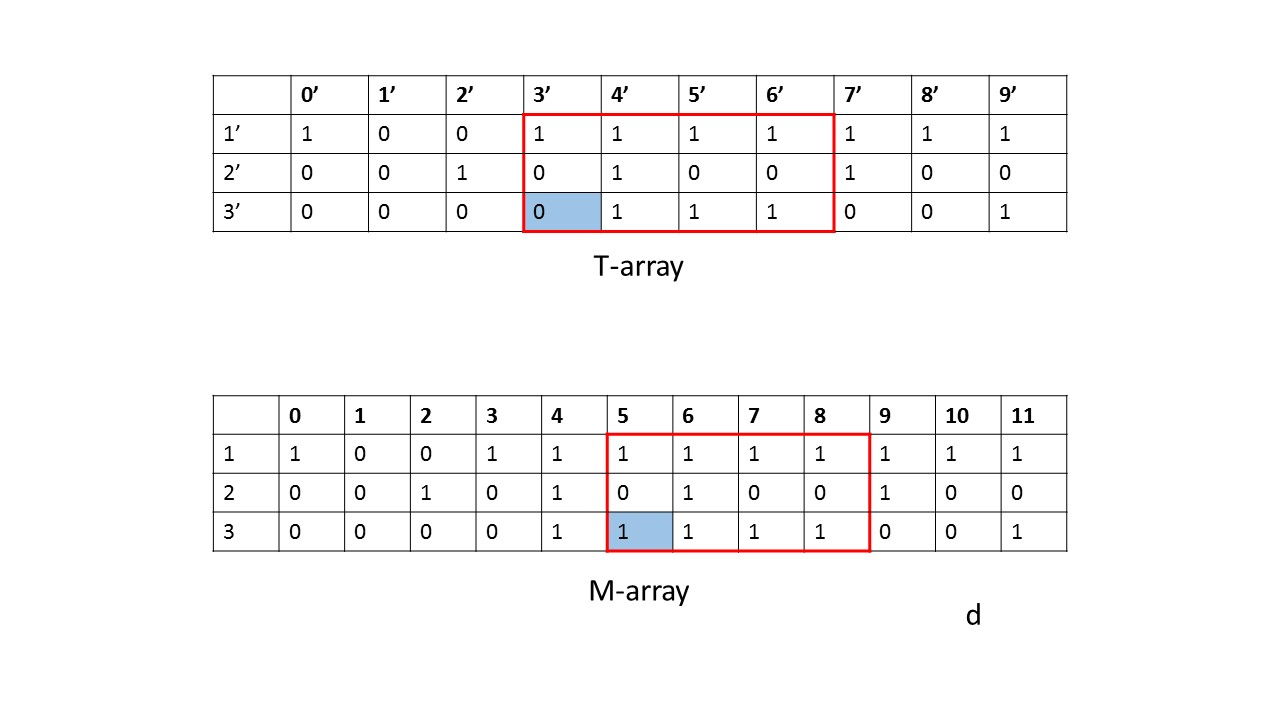
\includegraphics[scale=0.3]{fig/detect4.jpg}
     % \caption{Legend 4}
   \end{minipage}
	\caption{Detection of the disorders}
	\label{fig:detect}
\end{figure}


Then, as regions of the T-array extends because of the step 4, a new window can be initialized on the extended region and the growing starts again. At the end, except some array cells corresponding to dots lighted near the border of two objects, all the indices of the T-array have been determined.










\paragraph*{Detection of Pattern Disorders}
~~\\
Knowing that, in the T-array, the elements which still have no indices appear to be mostly alone or draw a chain, some rules permit to correct the index of these elements.

\begin{itemize}
\item if the element at the top and at the bot have the same index k, the current element has also this index k.
\item if the element at the left has the index k-1 and the one at the right k+1, then the current element has the index k.
\item the difference between the index of two horizontal neighbors corresponding to closer positions on the image is one.
\item if the indices of a consecutive vertical sequence are still undetermined, they get the index of the element at the top or bottom of the vertical.

\item if the indices of an consecutive horizontal sequence are still undetermined, they get the index such as it increases by one from index determined on the left to the on the right.
\begin{tabular}{|*{11}{c|}}
    \hline
     k-5  & k-4  & k-3  & \textcolor[rgb]{1,0,0}{k-2}  & \textcolor[rgb]{1,0,0}{k-1}  & \textcolor[rgb]{1,0,0}{k}  & \textcolor[rgb]{1,0,0}{k+1}  & k+2  & k+3  & k+4 & k+5 \\
    \hline
\end{tabular}
\end{itemize}

According to \cite{morita1988reconstruction}, the previous rules should correct the most of the errors of indexation and the cases where the error cannot be corrected are scarce.







\subsection{Grid Indexing}

The method of the binary M-array projection is based on the matching of a binary array, but other patterns can be used too to permit the matching of the projected and observed patterns. A non-exhaustive list of grid indexing is presented below.

\subsubsection{Mini-patterns Used as Code Words}

Instead of using a binary array, a technique can be using a array of words coded by patterns. Each pattern codes a word. As instance, on the figure \ref{fig:codeWords}, three words has been coded and permits to convert the projected pattern into a array of integers.


\begin{figure}[h]
  %\centering
  \centerline{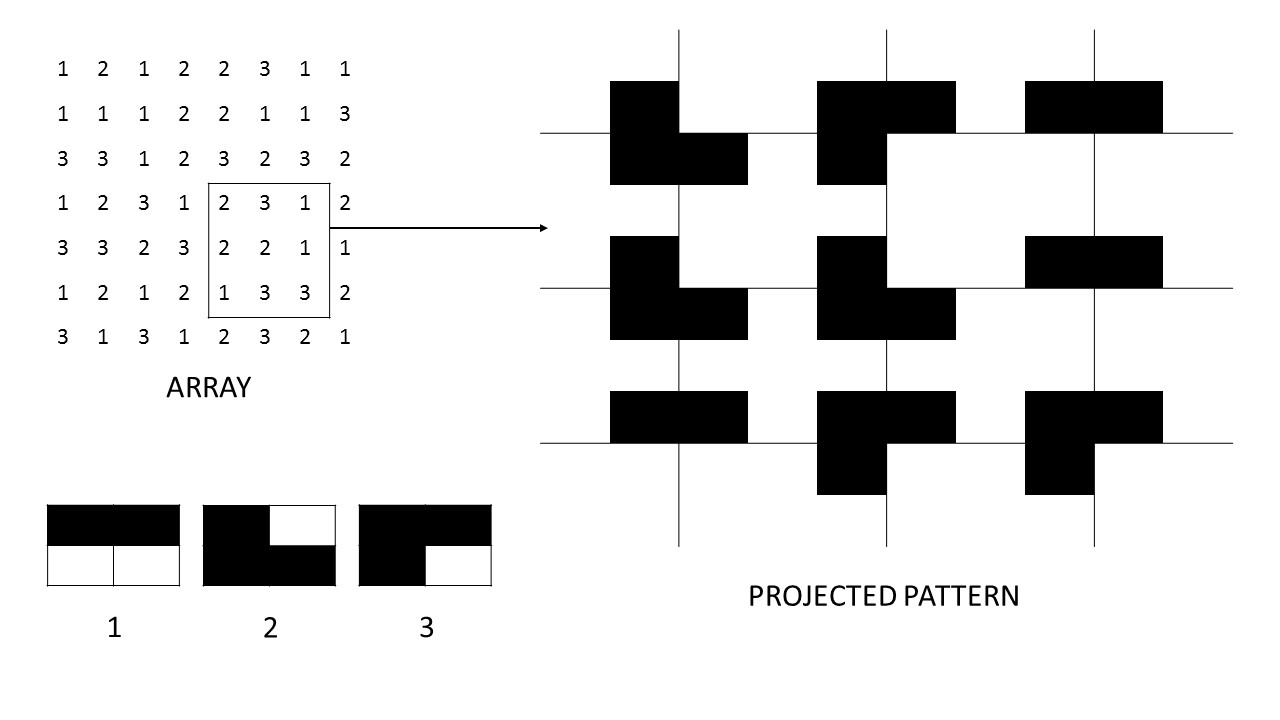
\includegraphics[scale=0.5]{fig/codeWords.jpg}}
  \caption{Mini-pattern used as code words}
  \label{fig:codeWords}
\end{figure}





\subsubsection{2D Array of Color-coded Dots}

Another technique is the 2D array of color-coded dots. The concept of this method is almost the same as the previous one but instead of using pattern to code a word, colors are used (see Figure \ref{fig:color-coded}).

\begin{figure}[h]
  %\centering
  \centerline{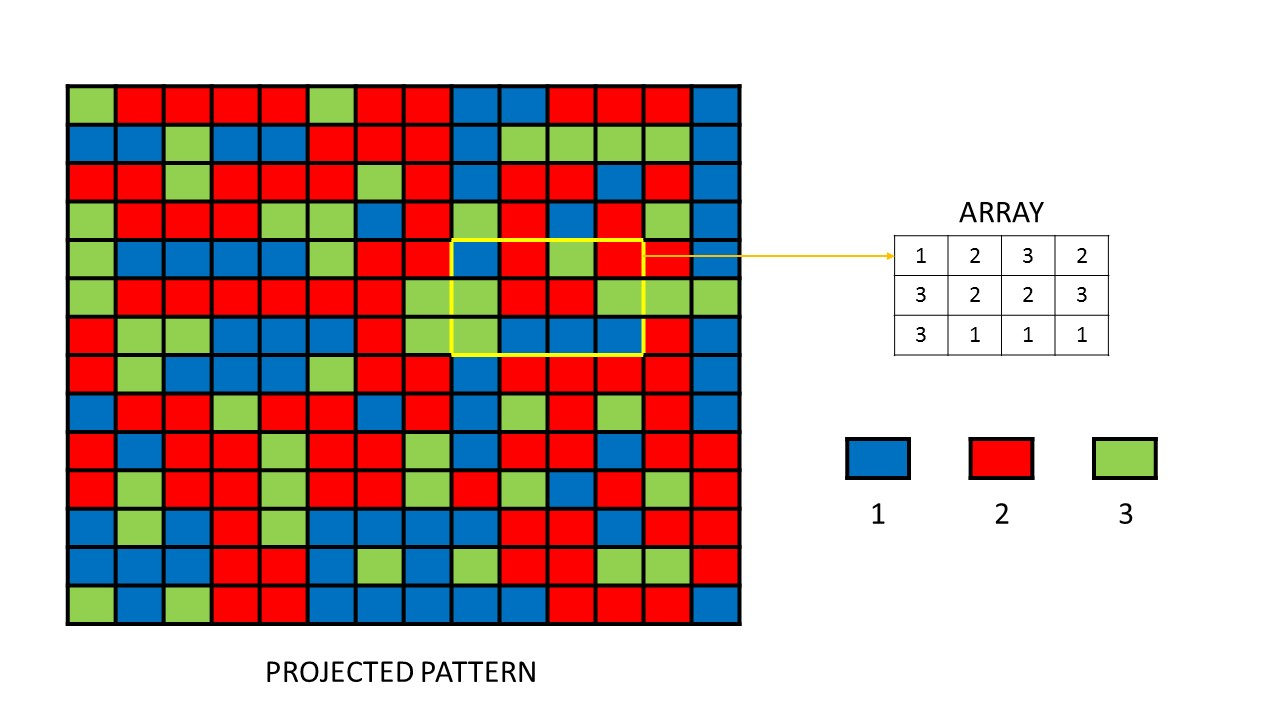
\includegraphics[scale=0.5]{fig/color-coded.jpg}}
  \caption{2D Array of Color-coded Dots}
  \label{fig:color-coded}
\end{figure}

\section{Artificial Light Source}
In order to carry out a 3D mapping of the target, the system needs a light source to project points which will be used by the 3D mapping algorithm. In this section, the source of light will be designed.

\subsubsection{Design of the Light Source}
~\\
First of all, the green has been chosen as color of the light source. Indeed, in order to detect easily the points projected on the target, a distinctive color should be used. As we can see figure \ref{fig:QeCCD}, the CCD selected for the camera has the best quantum efficiency for a wavelength around 510 $nm$, which means that the green is the color that is the best recorded by the camera. Secondly, as the surface on Mars is mainly orange, red and brown, this color should stand out.


\begin{figure}[h]
  %\centering
  \centerline{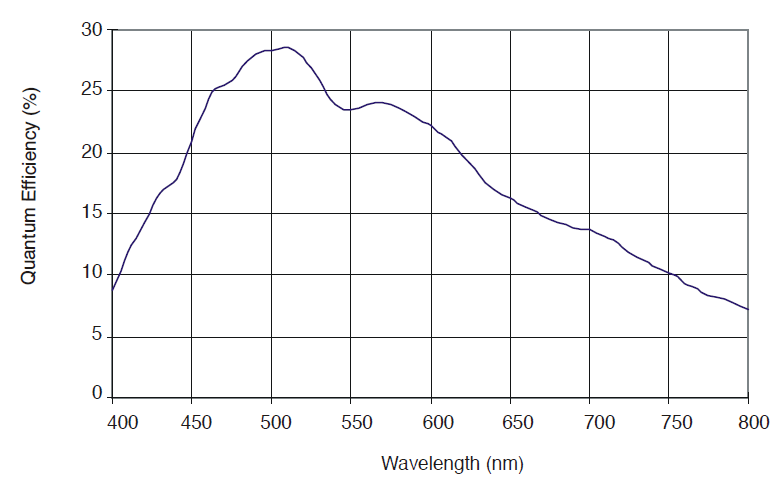
\includegraphics[scale=0.4]{fig/QeCCD.png}}
  \caption{Quantum efficiency versus wavelength of the CCD}
  \label{fig:QeCCD}
\end{figure}

Then, as only 300 $mW$ are available to aliment the light source and a lot of lightning energy is needed to outshine the sunlight, a LED has been chosen. Indeed, LEDs have great energy performances. The properties of the chosen LED can be seen in Annex \ref{LEDdatasheet}. Note that the use of a laser have been studied, but the energy cost would have been too expensive. Moreover, even if we cannot obtained a coherent light, as a laser do, with a LED, it is still feasible to obtain a monochromatic and directional light. Thus, we will assume that the LED can bring enough light (proof in part on Signal Noise Ratio\ref{light Power}).\
Then, as the 3D mapping algorithm needs a grid of points, the LED cannot be used in its present condition. Moreover, lot of light would be lost without an optic system. Thus, a system has been designed to concentrate the luminous beams of the LED and to transform the continuous light into a grid of point. The system uses a lens and a grid (Figure \ref{fig:LEDsystem}). 

\begin{figure}[h]
  %\centering
  \centerline{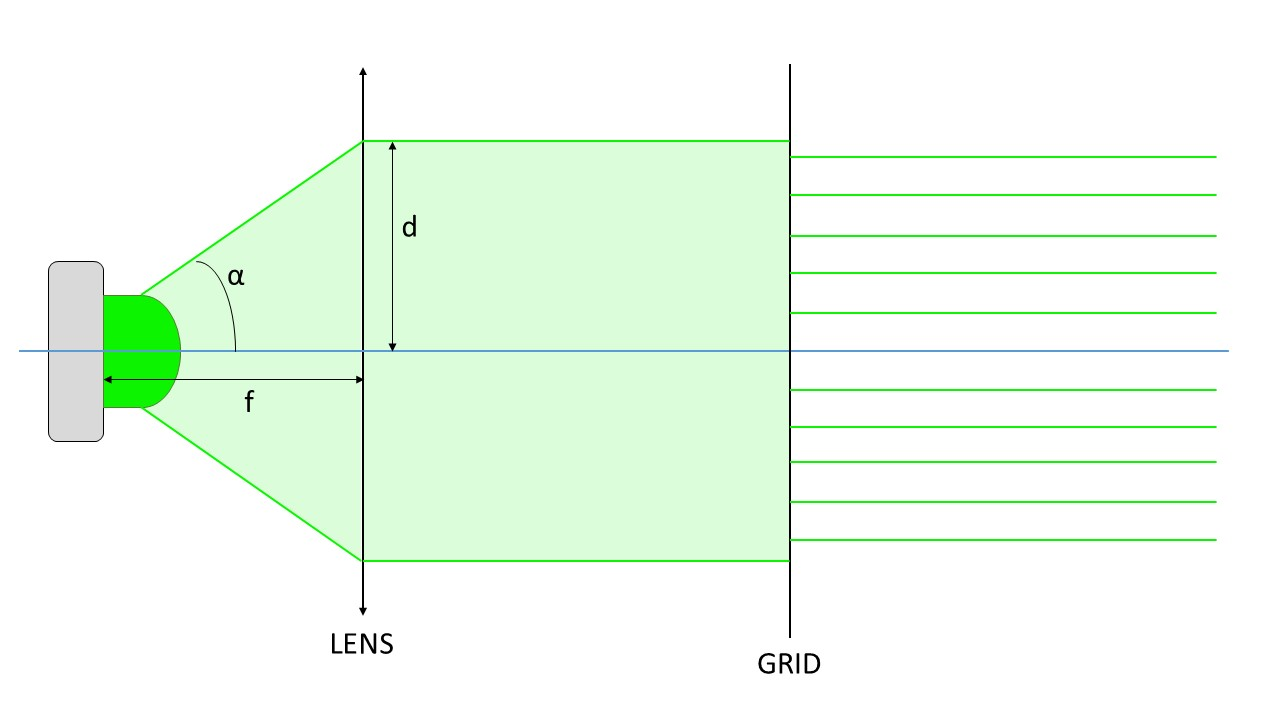
\includegraphics[scale=0.4]{fig/LEDsystem.jpg}}
  \caption{schema of the LED system}
  \label{fig:LEDsystem}
\end{figure}

As the LED has a diffusion angle of 30\textdegree (Annex \ref{LEDdatasheet}), the lens needs to be close enough to collect all the light beams of the LED to avoid losses of energy. In order to capture as much light as possible, the diameter of the lens should follow \eqref{eq:lenseLED}.

\begin{equation}
\label{eq:lenseLED}
d = f \tan \alpha
\end{equation}
with 
\begin{align*}
\alpha & = \frac{30}{2} = 15\mbox{\textdegree, the half of the diffusion angle.}\\
f & \mbox{, the focal length of the lens}
\end{align*}

Moreover, it should be pointed that there is a loss of energy because of the lens and the grid. We will assume that the energy loss coefficient of the lens $LFLLed$ (Loss Factor Lens Led) is 0.5 and the one of the grid $LFGLed$ (Loss Factor Grid Led) is 0.3.

\subsubsection{Validation of the Light Source}
\label{light Power}
~\\
In order to verify weather our light source has enough power or not to outshine the sunlight, the Signal/Noise ratio (SNR) has to be calculated (see part Signal/Noise ratio \ref{thirdcase}). Knowing that 100 is a really great SNR, as the SNR of images recorded with this system is $[32, 348]$, it can be concluded that the LED can be chosen as light source. Indeed, even if 32 is a low ratio, it is only when all the different poor conditions happen in the same time and it does not happen frequently. Moreover, 100 to 347are really high ratios that permit to have the 3D algorithm working well. Thus, the design of the light source is validated.





\section{Image processing}
In the following part of this report, the color detection will be used to distinguish color light points projected by a luminous source on a Martian rocks from its background. In order to implement this color detection, the HSV color model needs to be defined, as well as some morphological operations. 

\subsection{HSV Color System}
HSV stands for Hue Saturation Value. It is a color system which allows the separation of the color components from the intensity, unlike RGB system. It is more intuitive to find a plain object by varying HSV parameters.

The Hue designates the color itself. As it can be seen on the figure \ref{fig:HSV}, the color is determined by an angle between 0\degree and 360\degree. Red corresponds to 0�, green to 120� and blue to 240�. OpenCV range is 0-180. Changing the Saturation will affect the intensity of the color. A low value indicates a dull color. The Value has an impact on the luminosity of the color. Decreasing this value makes the color darker. The S and V are varying between 0 and 1 but the OpenCV range is 0-255.

\begin{figure}[H]
  \centering
  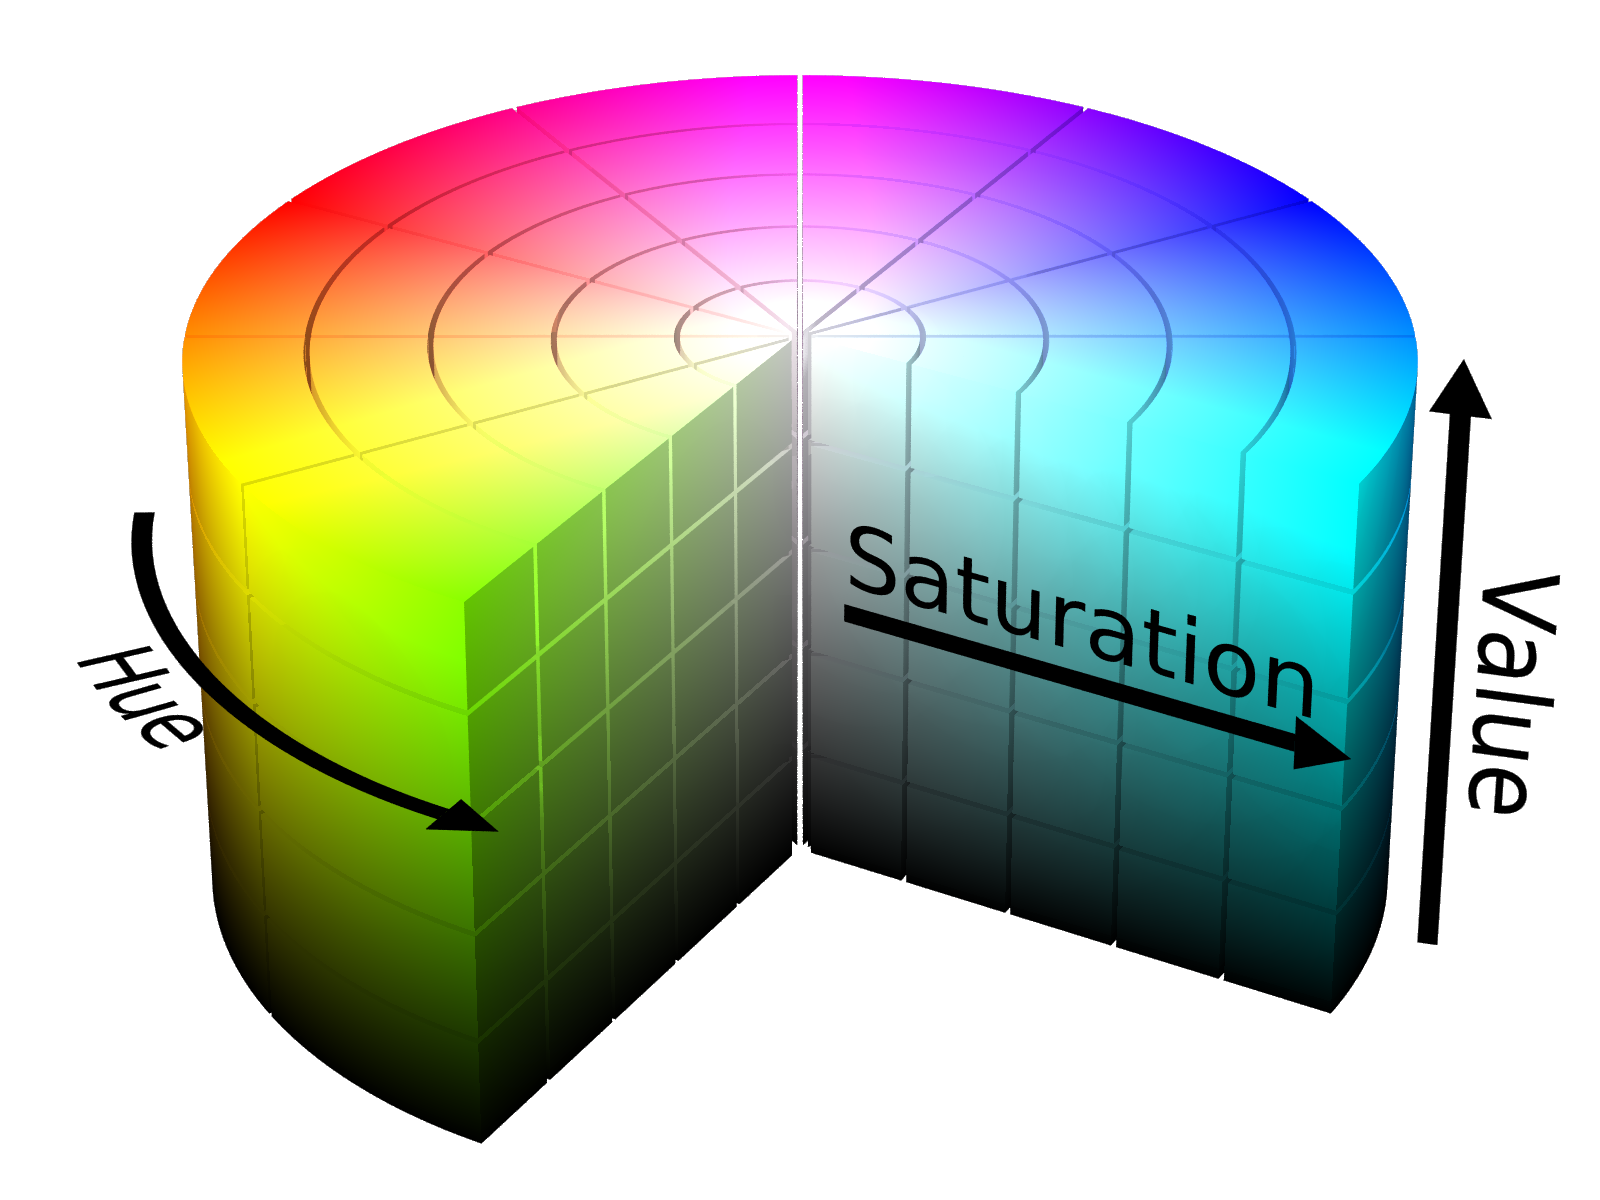
\includegraphics[scale=0.15]{fig/HSV.png}
  \caption{HSV diagram \cite{wiki:hsv}}
  \label{fig:HSV}
\end{figure}

\subsection{Morphological Operations \cite{bradski2008learning}}
The morphological operations on a binary image consists in applying a structuring element to each pixel of the object parts to reshape them. Two basic operations will be used later on and are explained here: the erosion and the dilation. Detailed diagram of the erosion and dilation can be found below (figures \ref{fig:erosion} and \ref{fig:dilation}). It should be noticed that for more legibility, the background is in white and the object in color. It will however be assumed that the pixels of the object have a value superior to the background.

\begin{figure}[h]
  \centering
  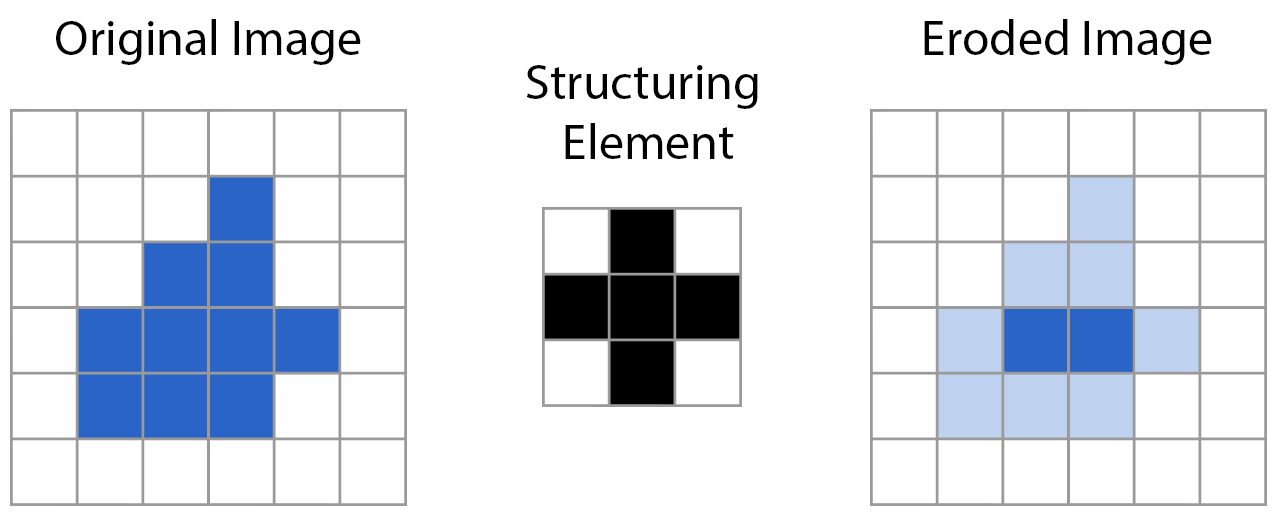
\includegraphics[scale=1]{fig/erosion.png}
  \caption{Erosion principle}
  \label{fig:erosion}
\end{figure}

\begin{figure}[h]
  \centering
  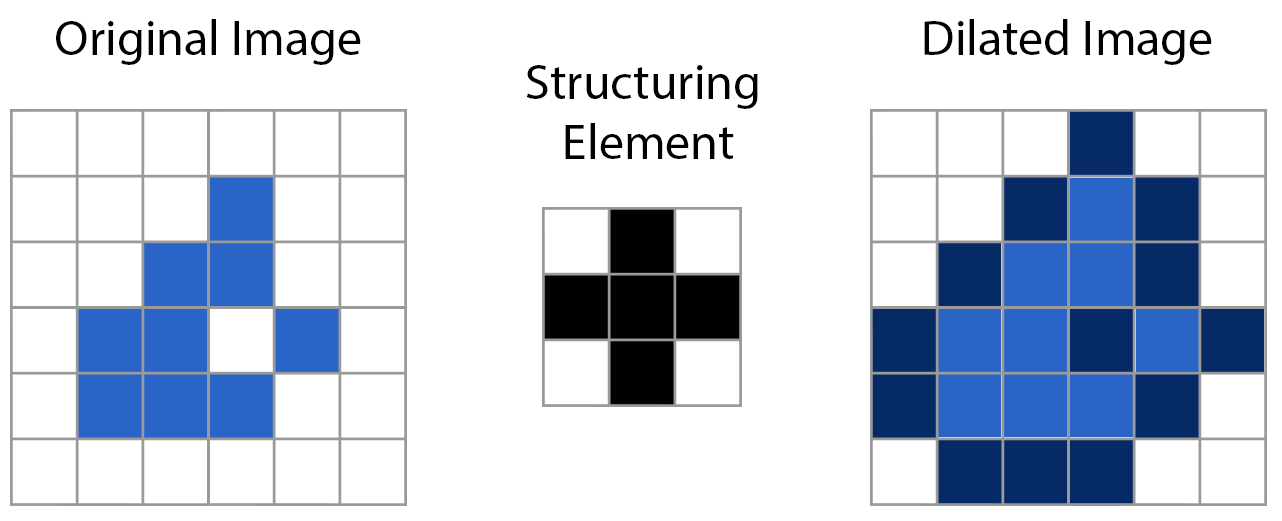
\includegraphics[scale=1]{fig/dilation.png}
  \caption{Dilation principle}
  \label{fig:dilation}
\end{figure}

\subsubsection{Erosion}
This transformation is similar to the logic gate AND. The structuring element or kernel is moved along the image and the minimal pixel value is set as the new value of the anchor point, in the figure, the center of the structuring element. This means that if all the points of the kernel are on an object (a white object on a black background), the anchor point will keep its value. On the contrary, if any element of the kernel is out of the object, the center point will become part of the background. The erosion is useful to separate two objects connected and to remove objects which are smaller than the size of the structuring element (noise). 

\subsubsection{Dilation}
The dilation is the opposite transformation of the erosion. It corresponds to the OR. If one element of the kernel is on the object (which is still assumed to have the maximal value for its pixel), the anchor point will be set to this value and thus be turned into a part of the object. This operation permits to fill holes in an object, to increase its size and to link objects which are closer than the size of the structuring element.

\subsubsection{Opening}
When combined, first by operating an erosion and then a dilation, the transformation is called an opening. The inverse operation is the closing. An opening could be convenient to separate luminous points which are connected and to then increase their size, lessen by the erosion to retrieve a shape similar to the original points.


\chapter{Development}
\section{Scene Analysis}
In order to design the camera and find its characteristics, a scene analysis have to be carried out. Our study is based on the MER (Mars Exploration Rover) cameras properties \cite{merengineeringcameras}.
To begin with, we choose an image sensor. 

\subsubsection{CCD}
\label{fig:CCD}
The Charge Coupled Device (CCD) is commonly more sensitive to light than its counterpart, the CMOS (Complementary Metal Oxide Semiconductor). Moreover, in the near infrared CCD appears to have a better response. Since Mars has a reddish color, it seems more accurate to select the CCD detector.

As scientists will need to discern the details of rocks, the resolution should be around the megapixel. Taking into account the cost, which will increase with the resolution, and the time of computation for an image with too many pixels, 1024 x 1024 seems to be an acceptable compromise.

Finally, the last element to consider is the pixel size. A trade-off have to be found between having a higher resolution (smaller pixels) and more sensitivity (larger pixels). All the camera of the MER mission were conceived with a pixel size of 12 x 12 $\mu m^2$ for a resolution of 1024 x 1024. It was decided to comply with that value.

For the next parts of this report, we will use the data sheet of the FTT1010M CCD image sensor (see Appendix \ref{CCDdatasheet}) as a basis for our calculations which will require CCD details.

\subsubsection{Field of View}
According to the book \cite{book}, the Field of View (FoV) \say{is the angle of the cone of directions encompassed by the scene that is being images}. This solid angle is needed to compute the focal length the camera should have.

\begin{figure}[h]
  \centering
  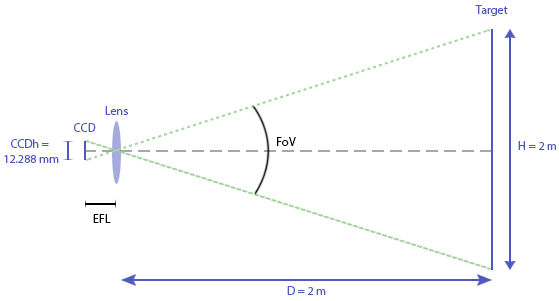
\includegraphics[scale=0.7]{fig/FOV.png}
  \caption{Field of View and Effective Focal Length}
  \label{fig:FOV}
\end{figure}

A simple relationship between the distance lens-target, the size of the target and the FoV can be deduced from the detailed diagram \ref{fig:FOV}: 
\begin{equation*}
tan( \frac{FoV}{2}) = \frac{1}{2} \times \frac{H}{D}
\end{equation*}
We derive and get
\begin{equation*}
 \frac{FoV}{2} = atan(\frac{1}{2} \times \frac{H}{D})
\end{equation*}

Numerically, with our problem delimitation, the Field of View is equal to $26.6\degree \times 26.6\degree$. 

\subsubsection{Focal Length}
\label{focalLength}
Thanks to the previous diagram, the Effective Focal Length (EFL) can also be determined: 
\begin{equation*}
EFL = \frac{1}{2} \times \frac{CCDh}{tan(\frac{FoV}{2})} = 12.29 \ mm
\end{equation*}
where $CCDh$ is the image section of the CCD according to the data sheet.\\

In order to get the real focal length, we choose $rf = 1 \ m$ for the distance of focus of the camera. 
\begin{equation*}
f = \frac{1}{\frac{1}{rf}+\frac{1}{EFL}} = 12.14 \ mm
\end{equation*}

\subsubsection{Aperture}
\label{aperture}
To determine the diameter of the aperture, several criteria have to be accounted for. If the diameter is too small, the sharpness of the image will decrease due to the diffraction effect. In fact, at large aperture, the diffracted light is negligible compared to the total amount of light entering the system. On the other hand, we should also consider the Depth of Field (FoV). We need to insure that it is big enough to allow us to see the whole target on the image. The relationship between the DoF and the diameter is inversely proportional. That means that if we increase the diameter, we will lessen it. The Diameter of Confusion (DoC), linked to the DoF is also a factor to take into consideration for the choice of the diameter. According to Wikipedia \cite{wiki:coc} It corresponds to \say{an optical spot caused by a cone of light rays from a lens not coming to a perfect focus when imaging a point source}. The smaller the DoC is, which corresponds to a better focus, the bigger is the DoF, and also the smaller is the diameter.

As the behaviour of the depth of field and of the diameter of confusion runs counter to the diffraction one, a trade-off has to be found. 

These formula are used to calculate the diameter of confusion and the diffraction spot:
\begin{equation*}
DoC = Dsr \cdot \frac{|r-rf|}{r} \cdot \frac{f}{rf - f}
\end{equation*}
where $Dsr$ is the diameter of the aperture
\begin{equation*}
DiffractionSpot = 2 \cdot EFL \cdot tan(1.22 \cdot \frac{lambda}{Dsr})
\end{equation*}
where $lambda$ is a wavelength of the sunlight\\

In the delimitations, it is assumed that the wavelengths of the sunlight belong to [400 800] nm. To settle on a diameter, the diameter of confusion and the diffraction spot were computed for diameters varying from 1 mm to 5 mm and wavelengths from 400 nm to 800 nm. The results are shown graphically in figure \ref{fig:DoCDifspot}. As the diameter of confusion cannot be bigger than the height of a pixel, the line corresponding to 12 $\mu m$ was also added to the graphic. In order to have the best trade-off, that is to say all the curves under 12 $\mu m$, we have chosen a effective lens entrance aperture $Dsr$ equal to $1.9 \ mm$, corresponding to $DoC = 0.0117 \ mm$. 

\begin{figure}[H]
  \centering
  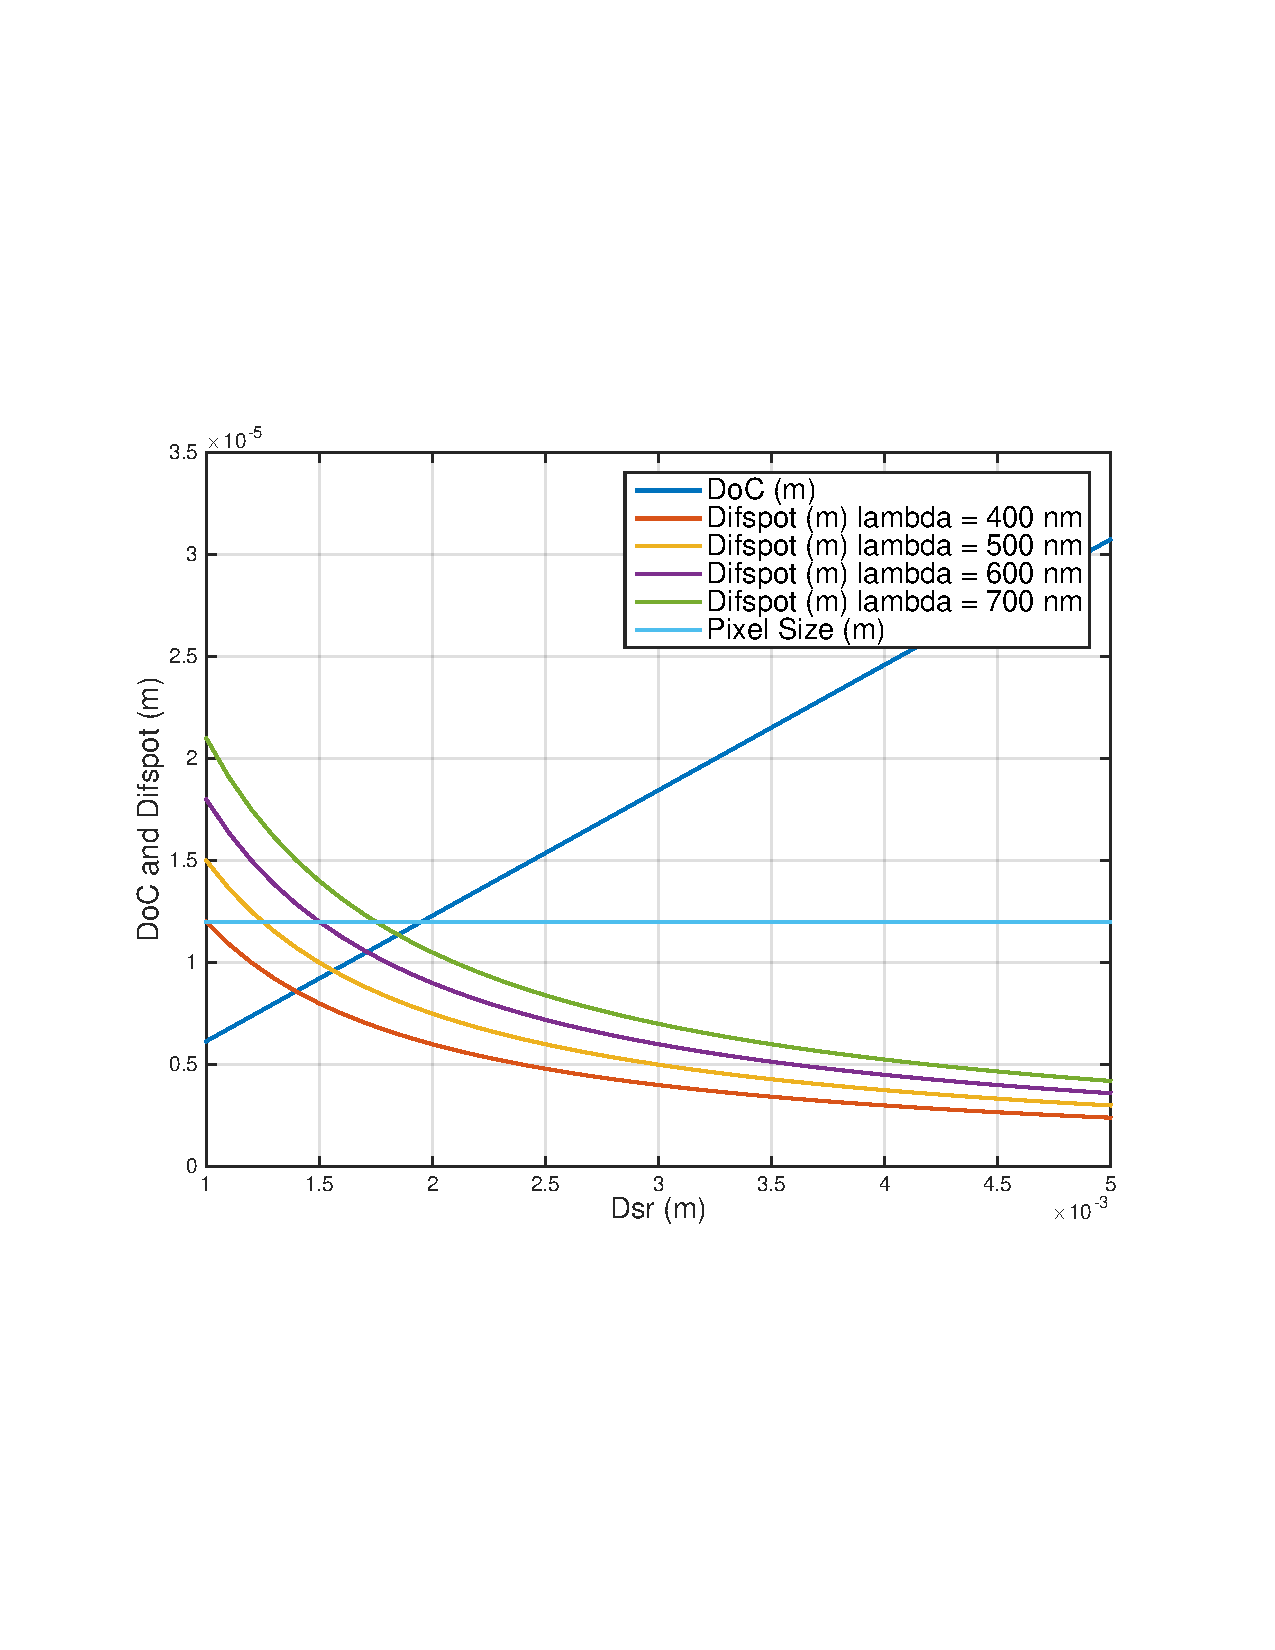
\includegraphics[trim=2cm 7cm 2cm 7cm, clip=true, totalheight=0.45\textheight, angle=0]{fig/DoCDifspot.pdf}
  \caption{Diameter of confusion and diffraction spots as a function of the diameter}
  \label{fig:DoCDifspot}
\end{figure}

Then, the depth of field can be deduced:
\begin{equation*}
DoF = \frac{2\frac{f}{Dsr}DoC(m+1)}{m^2 - (\frac{DoC}{Dsr})^2} = 1.33 \ m
\end{equation*}
That means that the roughness of the rock analysed cannot be more than $\frac{DoF}{2} =  66.5\ cm$ since we could not see the whole rock if not, and the 3D map will then be flawed.
First of all, the irradiance $F$ of the light from the sun falling at the top of the atmosphere of Mars can be calculated as following :
Conservation of energy :
\begin{equation}
\label{eq:conservation of energy}
4\pi R_\odot^2F_\odot=4\pi R^2F
\end{equation}
with 

$R_\odot=6,956.10^8\ m$ : solar radius

$F_\odot=6,45.10^7\ W.m^{-2}$ : energy flow of the surface of the sun

$R \in [2.06644,\ 2.49228].10^{11} \ m$ : distance Mars-Sun (Aphelion and Perihelion)

\begin{equation}
\label{eq:Irradiance Sun range}
F = F_\odot \left(\frac{R_\odot}{R}\right)^2 \in [502, 730]\ W/m^2
\end{equation}

In this report, we will consider that the rover is working on a specific date and we will chose the one when $R$ corresponds to the semi-major axis. In this case $R=2,27936.10^{11}\ km$ and
\begin{equation}
\label{eq:Irradiance Sun}
F = 589\ W/m^2
\end{equation}



Moreover, we can assume that a part of the irradiance is absorbed by the atmosphere. Knowing that the atmosphere of Earth absorbs and scatters to space around 30\% of the incident irradiance of the Sun\cite{yamamoto1962direct}, and knowing  that the atmosphere of Mars is thinner than the one of the Earth, we will postulate that 10\% of the incident irradiance is absorbed. Thus, using \ref{eq:Irradiance Sun} the actual irradiance $F_a$ of the light from the sun falling on the surface of Mars is

\begin{equation}
\label{eq:Actual Irradiance Sun}
F_a = \frac{90}{100}F = \frac{90*589}{100} = 530\ W/m^2
\end{equation}

However, this irradiance is the one of surface exposed perpendicular to the sun's beams. As Mars is a sphere, the projection need to be considered.
Knowing that the weather is better into the northern hemisphere of Mars\cite{wiki:weather} and the fact that a latitude between 30 an 70 degrees is favored for a landing\cite{latitude}, we will assume that the rover has a latitude of 50\textdegree. This latitude corresponds to an angle of 40\textdegree$\ $between the surface of Mars and the sun's beams. Moreover, suppose that the rover stop working when this angle is inferior to 10\textdegree. Thus, the irradiance $F_{50}$ at a latitude of 50\textdegree$\ $is

\begin{equation}
F_{50} = F_asin(angleBeams) \in [92, 341] \ W/m^2
\end{equation}

with $angleBeams = [10, 90-latitude] = [10, 40]$\textdegree.


Then, considering the trajectory of the Sun into the sky of Mars and knowing that the rock target is more or less vertical to the surface of Mars, the angle $\theta$ between the target's normal and the sun's beam is considered to be included in $[10, 50]$\textdegree. In addition, in the optimal case (when all the optimal conditions are provided to have the maximal radiance), the BRDF of the surface of the target is assumed to be 90\% Lambertian and 10\% Glossy while in the worst case the BRDF will be only Lambertian. In this way, the radiance of the target $R_T$ is

\begin{equation}
\label{eq:Radiance Target}
R_T = \left\{
	\begin{array}{ll}
		\frac{F_{50}\alpha}{\pi}\cos \theta & \mbox{ optimal case} \\
		F_{50}\alpha(\frac{9}{10\pi}\cos\theta + \frac{1}{10}) & \mbox{ worst case}
	\end{array}
\right.
\end{equation}

with 
\begin{align*}
	\alpha & \in [0.05, 0.45]\mbox{, the albedo of the target\ref{albedo}} \\
	\theta & \in [10, 50]\mbox{\textdegree, the angle between the target's normal and the sun's beam}
\end{align*}
Thus, 
\begin{equation}
R_T \in [92, 340] \ W/m^2
\end{equation}






\subsection{Summary and Comparison with MER Cameras}
To validate the coherence of the characteristics of the designed camera, a comparative table \ref{tabCameras} with the MER cameras Navcam (Navigation Camera) and Pancam (Panoramic Camera) \cite{merengineeringcameras} can be found below.

\begin{table}[H]
\centering
\caption{Recap chart of the Designed Camera and Comparison with Navcam and Pancam (MER Cameras)}
\label{tabCameras}
\renewcommand{\arraystretch}{1.5}
\begin{tabular}{|l|c c c|}
\hline
Features & Designed Camera & Navcam & Pancam \\
\hline
CCD &  &  &  \\
Pixel size & $12 \times 12 $ microns & $12 \times 12 $ microns & $12 \times 12 $ microns \\ 
Resolution & $1024 \times 1024 $ & $1024 \times 1024 $ & $1024 \times 1024 $ \\ 
Spectral range & [400 - 800] nm & [600 - 800] nm & [400 - 1100] nm \\ 
Readout noise, 55$\degree$ & 25 electrons & 25 electrons & 25 electrons \\
\hline
Optical properties & & &  \\
Focal length & 12.14 mm & 14.67 mm & 43 mm  \\
Entrance pupil diameter & 1.9 mm & 1.25 mm & 2.18 mm  \\
FOV & $26.6 \degree \times 26.6\degree$ & $45 \degree \times 45\degree$ & $16 \degree \times 16\degree$ \\
Depth of field & 0.67 - 2 m & 0.5 m - infinity & 1.5 m - infinity \\ 
Best focus & 1 m & 1 m & 3 m \\
\hline
\end{tabular}
\end{table}

The CCD parameters are similar except for the spectral range. As Pancam mission is to investigate Mars terrain and obtain color images of any information useful to learn more about the Red Planet, that seems logical that the spectrum is wider than the one we choose. The navigation camera provides a 360$\degree$ view of the area where is located the rover. The spectrum was reduced using filters to allow a higher spectral responsivity.
For the optical features, it can be noticed that the parameters have approximately the same size. The depth of field for our camera is restricted but it is due to our aim: stabilizing the camera in front of a rock and carrying out its depth map.
We can conclude that since the MER cameras accomplish well their task, the designed camera which is comparable to them should also be capable of acquiring good images on Mars.

\subsection{Cost and Power Consumption}
The price of a camera depends of its characteristics, especially, of the CCD sensor. The chosen one has large pixels and hence will capture more light than another CCD with half of our pixel size. That means that its performance should be better and thus, the designed camera could be quite expensive. As the exact cost of high quality camera is often not provided, and as finding a similar model to the one planned above is very difficult, it is decided to only determine a price range. Some websites such as ThorLabs have CCD cameras with a resolution of one Megapixel but with half the pixel size desired. As their cost is between 5.000 and 9.000 \euro, we estimate our camera at around 10.000 \euro. Knowing that the Nasa has planned a budget of \$1.5 billion for the new Mars Rover Mission of 2020, this price represents only $0.73\cdot 10^{-3} \ \%$ of the total mission. Taking into consideration that the fee for the artificial source (LED and lens) is negligible compared to the camera cost, it can be concluded that the amount of money needed for buying the designed camera is reasonable.

Regarding the power consumption of our system, it is assumed that the camera could be powered with 2.15 Watts since it is sufficient for supplying the MER Cameras. On the other hand, according to its datasheet (Appendix \ref{LEDdatasheet}), the LED consumption is of 220 mW. On the report of the NASA, a Martian rover needs around 100 Watts and they are provided by solar panels and rechargeable Lithium batteries. The system will then use around 2.4 \% of the rover power. It is tolerable since the camera will not take pictures all the time. It can be argued that the processor consumption should be added. However, the other actions of the robot are also controlled by the CPU, so it is not taken into account here, since it is hard to quantify the power utilized by the algorithms to compute the depth mapping.
\section{Distance Camera-Target of One Point}
Before starting to establish a whole 3D mapping, a more simple case can be studied first and it will be shown, in this section, how to determine the distance to only one point. Indeed, the distance between the camera and a point of the target can be easily determined thanks to a little bit of trigonometry.

The context of this case is simple, the camera is recording images of the target while the artificial light source is projecting a point one the last one (see figure \ref{fig:schema1D}).

\begin{figure}[h]
  %\centering
  \centerline{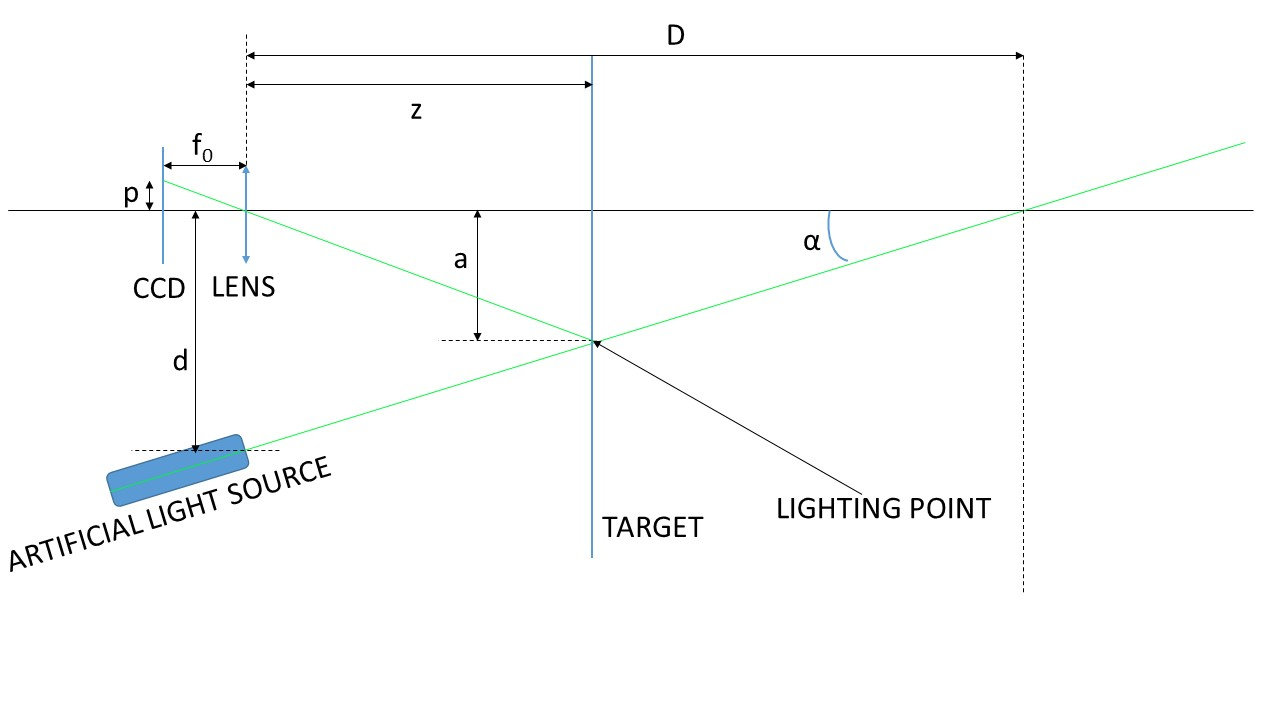
\includegraphics[scale=0.5]{fig/schema1D.jpg}}
  \caption{schema of the camera recording images of the target on which there is a lighting point from the artificial light source}
  \label{fig:schema1D}
\end{figure}

According to the figure \ref{fig:schema1D}, 
\begin{itemize}
\item \textbf{d} is the distance to determine.
\item $\bm{\alpha}$ is the angle between the focal axis of the camera and the focal axis of the light source.
\item \textbf{a} is the distance between the focal axis of the camera and the lighting point.
\item \textbf{D} is the distance between the camera and the lighting point when this one is on the focal axis of the camera.
\end{itemize}
Thus, we have

\begin{equation*}
	d=D-\frac{a}{\tan \alpha}
\label{eq:formule_1D}
\end{equation*}

However, $\bm{\alpha}$, \textbf{a} and \textbf{D} are not known yet, that is why a calibration phase is needed (see Figure \ref{fig:calibration}). The first parameter, $\bm{\alpha}$, is determined during the installation of the light source and the camera on the rover. Then, during the calibration, two steps can be identified. During the first one, a target is positioned such as the lighting point is on the center of the image recorded by the camera. Thus, \textbf{D} can be measured. During the second step, a target is positioned such as the lighting point is right on side (left or right) of the image recorded by the camera (see Figure \ref{fig:calibration}). Therefore, $a_0$ can be measured and we have

\begin{equation*}
	a = \frac{Na_0}{A_0}
\end{equation*}


with \begin{itemize} \item $N\ [pixels]$, the number of pixel between the center of the image recorded by the camera and the lighting point.
\item $A_0$ $[pixels]$, the number of pixel between the center of the image recorded by the camera and the lighting point during the calibration phase, that is to say, the half of the pixels of the width of the image.
\end{itemize}

Therefore, we have
\begin{equation}
	d=D-\frac{Na_0}{\tan \alpha}
\label{eq:formule1D}
\end{equation}

\begin{figure}[H]
  %\centering
  \centerline{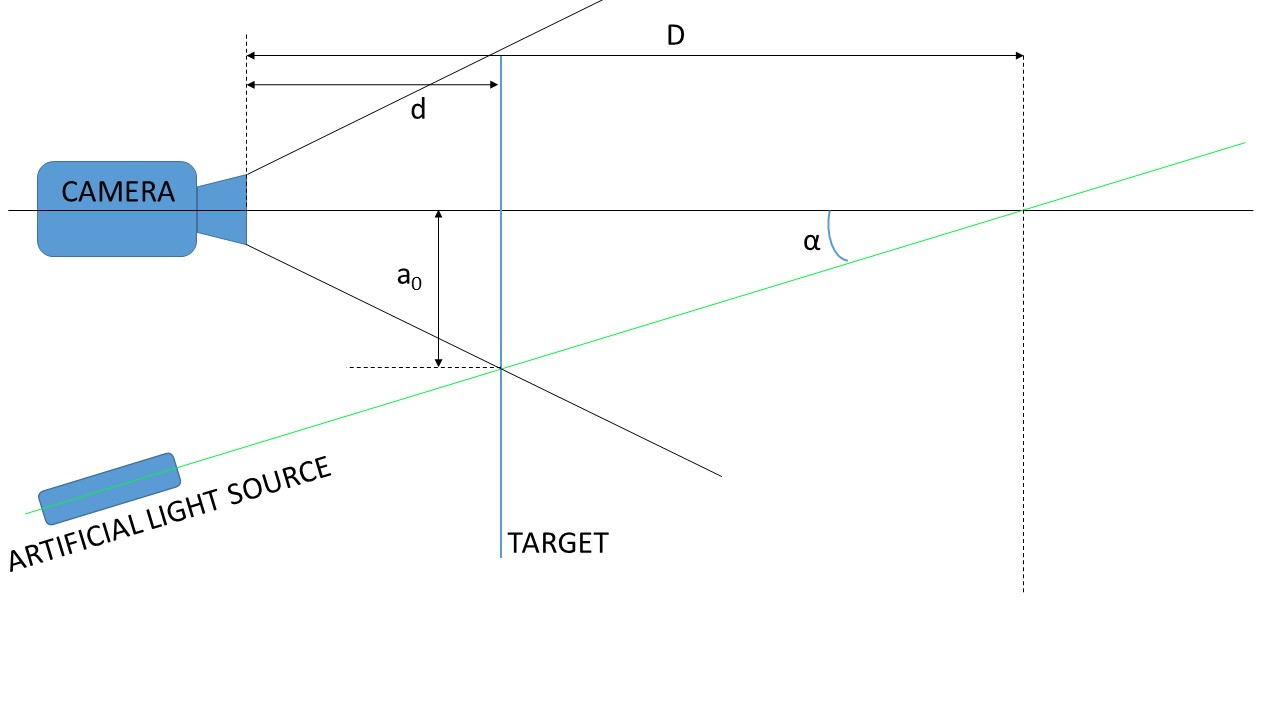
\includegraphics[scale=0.4]{fig/calibration.jpg}}
  \caption{schema of the calibration}
  \label{fig:calibration}
\end{figure}


However, a calculation of the distance camera - target using simpler calibration can be found thanks to triangulation. Indeed, using the Thales' theorem such as $\frac{z}{f_0} = \frac{a}{p}$ (see Figure \ref{fig:schema1D_2}), it can be determined that the distance \textbf{z} camera - point on the target is


\begin{equation}
z = \frac{f_0d}{p+f_0 \tan \alpha}
\label{eq:formule1D_2}
\end{equation}

Thus, only the first step of the calibration is needed because only $\bm{\alpha}$ and \textbf{d} need to be determined. $\bm{f_0}$ is a characteristic of the lens and \textbf{p} is determined thanks to the CCD characteristics ($p = p_{pixels} \frac{12,288.10^{-3}}{1024}$).

\begin{figure}[H]
  %\centering
  \centerline{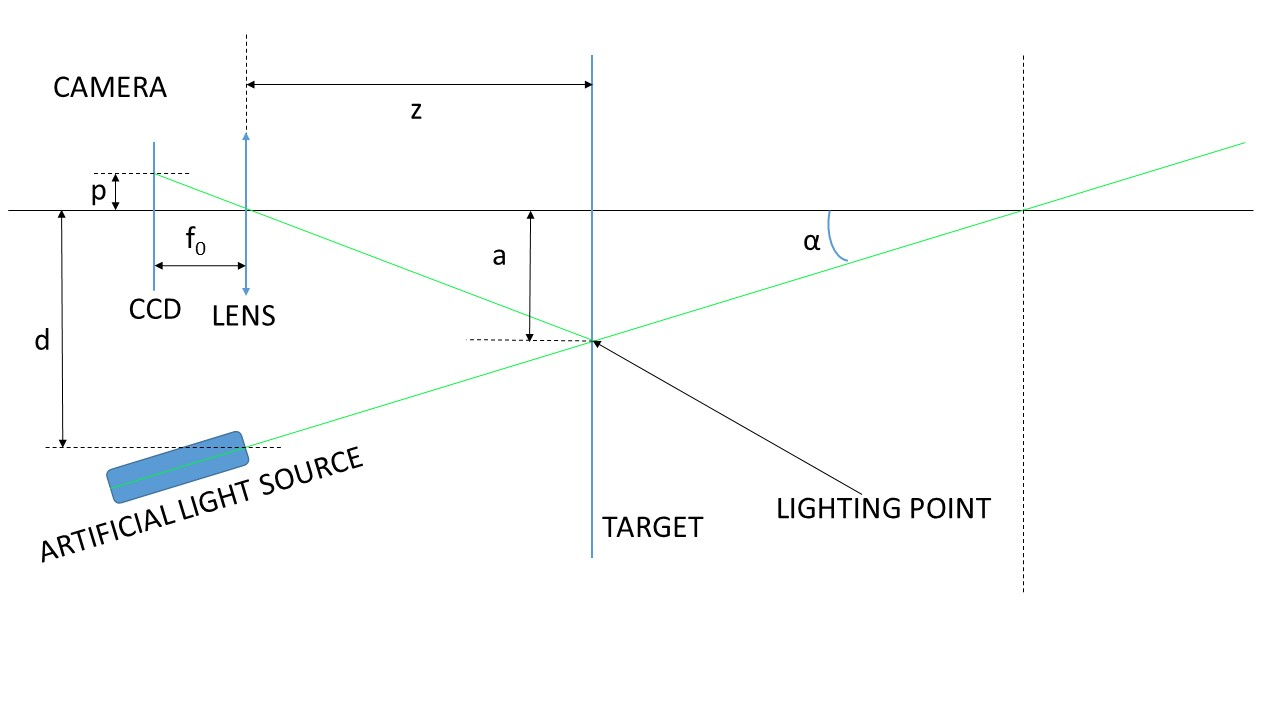
\includegraphics[scale=0.5]{fig/schema1D_2.jpg}}
  \caption{schema of the CCD sensor - lens sytem recording images of the target on which there is a lighting point from the artificial light source}
  \label{fig:schema1D_2}
\end{figure}
\section{Image Processing}
To carry out the 3D map of a Martian rock, the coordinates of the points which are projected by the LED on its surface need to be determined on the images acquired by the camera. They are obtained by detecting the points thanks to their color, by distinguishing them, and by applying the centroid algorithm to get their center. First, the color detection method will be addressed, before focusing on the differentiation and the centroiding.

\subsection{Color Detection}

To increase the robustness of the algorithm, the color of the light beams was chosen to have the maximum contrast with the color of the rock. Mars having a reddish color, a bright green light seemed adapted. Moreover, as it is explained in the scene analysis part, the CCD sensor is more sensitive to the wavelength corresponding to the green (around 520 nm). Thus, the color detection algorithm aims to find bright green spots in the camera video stream in real time. It is implemented in C with OpenCV library. 

For unit testing, the image analysis is performed by extracting frames from the video stream obtained thanks to the computer webcam. These images are processed very quickly, which allows a real time analysis. The details of the method employed are given below. For the explanation, the figures are obtained for the detection of a blue box (the H value was changed for this purpose), but the algorithm works similarly for green light beams.

To begin with, a low-pass filter is applied to the image to handle to smooth it and to reduce the noise. Once achieved, the image is converted from RGB to HSV (see Theory Section) in order to get a better control of the colors and intensities of the image pixels. The range of the HSV parameters can be determined to isolate the bright green pixels from the rest of the image. The equivalent hue is between 60\degree  and 180\degree, taking a large scope to be sure to isolate the good color component. As the luminous points will be bright, the range of the saturation and the luminosity should be chosen around the upper values. To adjust the values, several trackbars are added to the image, see figure \ref{fig:trackbars} and the modifications are made in real time. All the values under the thresholds defined are irrelevant. Thus the pixels of the binary image which corresponds to the HSV thresholding are set to 1 (white) for the zone where the light green points are recognized and to 0 (black) for the background, the rest of the image. This image is then easier to deal with because it is only composed of two values, black and white. Erosions and dilations can be applied respectively to separate connected light beams and remove noise or to fill holes in the points. The number or erosions and dilations are selected thanks to trackbars once again (figure \ref{fig:trackbars}) and they are computed with the OpenCV functions with a 3x3 rectangular structuring element. The size of the kernel of the low-pass filter is also controllable with the trackbars. 

\begin{figure}[H]
  \centering
  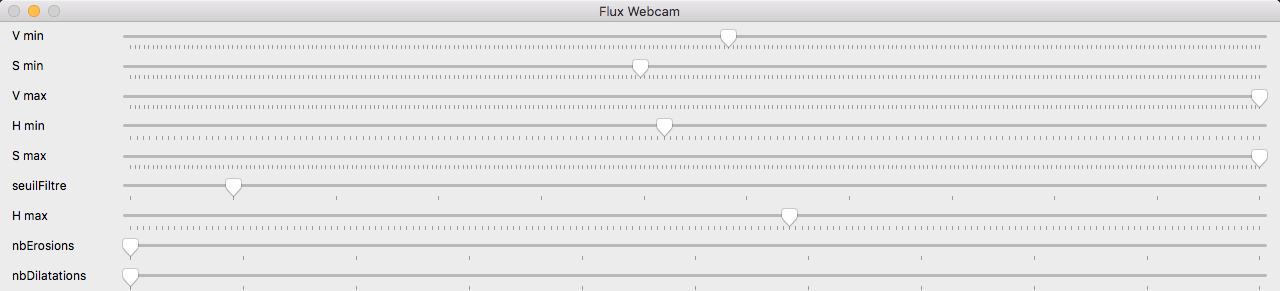
\includegraphics[scale=0.35]{fig/trackbars.png}
  \caption{Trackbars for the threshold of the filter, the HSV parameters and the number of erosion and dilation}
  \label{fig:trackbars}
\end{figure}

The calibration is carried out through the trackbars and the result is displayed on the video stream with the addition of contours to facilitate the tuning (figure \ref{fig:contours}). \textit{cvFindContours} is used to search the contour of the light spots. The detection is based on the same principle that it has been seen during the exercises in the lab. The algorithm looks for the first pixel belonging to the point and then follows the contour pixel by pixel. Once the threshold of the low-pass filter, the HSV values and the number of erosion and dilation are established, the calibration is completed. For the unit testing with the blue box, we only focus on the color detection and the centroiding. Thus, no erosion nor dilation are added and the filter kernel is set to one pixel, which does nothing. 

\begin{figure}[H]
  \centering
  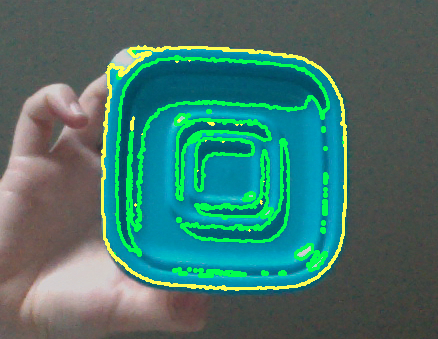
\includegraphics[scale=0.6]{fig/contours.png}
  \caption{Contours of the detected object}
  \label{fig:contours}
\end{figure}

In order to compute the centroid of the beams spots, it is needed to retrieve their intensity. To this end, the color detection should return an image with the light points in HSV color on a black background. To do so, the binary image is multiplied by the HSV image. The multiplication is explained by the pseudo code below.\\

\begin{algorithmic}
\Function{multiplication}{binary image, color image}
	\For{each pixel in the binary image}
		\If {the pixel value is white}
    			\State $pixelHSVColor \gets$ the color of the pixel in the HSV image
    			\State the color of the pixel in the final image $\gets pixelHSVColor$
		\Else
        			\State the color of the pixel in the final image $\gets$ black color
		\EndIf
	\EndFor
\EndFunction
\end{algorithmic}

The final image obtained is shown figure \ref{fig:finalImage}. Each white pixel corresponding to 1 in the binary image is replaced in the final image by the HSV value of the original image and the background is set to black like in the binary image.

\begin{figure}[h]
  \centering
  
\includegraphics[scale=0.6]{fig/finalImage.png}
  \caption{Object detected in HSV color system on a black background}
  \label{fig:finalImage}
\end{figure}

\subsection{Beams Distinction}
In the previous part, a unit test was performed with a blue box to check the efficiency of the color detection algorithm. However, the aim is to project a grid of 10 x 10 green points on a rock. Once they are extracted from the rest of the image with the same technique described above, they need to be separated. Indeed, for now, we only have the coordinates of the pixels assumed to belong to the beam spots. To look for their center of mass, the pixels which constitute each point have to be gathered. 

It should be noticed that, as no pattern other than an unicolor grid is used to carry out the depth mapping, the green points cannot be distinguished from each others. Thus, this implementation does not take into account the position of each beam spot, which could be problematic if the deformation is too important. Indeed, if a point is slightly linked to another or if it has moved and is a bit above or under the others, it is still possible to retrieve its original position. It is only if the change is too important (permutation of dots for example), that it will be very complicated to get the correct location of each beam spot. To solve this problem, a solution is described in the Pattern Disorders paragraph \ref{PatternDisorders} in the Theory Section, which would assure that no spot has been switched. Nevertheless, this method requires a pattern projection and is dismissed in a first approach. 

To differentiate each point, a recursive method was implemented using C++ which consists to isolate a point using neighbouring pixels. The pseudo code explaining the technique can be found below:\\

\begin{algorithmic}
\Function{findPointRec}{table, pixel, information to scan the image}\\
\Comment{table contains the coordinates of the pixel belonging to the current point}
		\If {the pixel value is is not black}
    			\State add to $table$ the $pixel$ coordinates and its value
    			\State the $pixel$ value in the image $\gets$ 0
			\State findPointRec(table, left neighbouring pixel, image information)
			\State findPointRec(table, right neighbouring pixel, image information)
			\State findPointRec(table, above neighbouring pixel, image information)
			\State findPointRec(table, below neighbouring pixel, image information))
		\EndIf
\EndFunction
\end{algorithmic}

The image is scanned and it is assumed that a new point begins each time that a green pixel is detected. A table to collect the coordinates of pixels belonging to the new beam spot is created and given in parameter to the recursive method. The first pixel position is added to the table, its value is set to 0 in the image and the recursive method is repeated while neighbouring pixels are found. At the end, a 2D table is obtained where the rows correspond to the spots and the columns to each pixel belonging to the point. The centroiding algorithm can then be processed to determine the center of mass of each spot and compute their distance to the camera. We can note that, for now, the points are separated but if they were not perfectly aligned on the projection, the rows of the 2D table are not in the same order than the original projected points.
\subsection{Centroiding}

The 3D map can be performed with the coordinates of the light beams seen by the camera. They are determined by estimating the center of the spot, and to do so, the center of mass, also called the centroid needs to be calculated in the final image acquired by the color detection. In order to get it, a barycenter of the pixels belonging to the ray is carried out weighted by the intensity of the pixel (S value in HSV model).

\begin{align}
x_c &= \frac{\sum_x x \cdot I(x,y)}{\sum_x \sum_y I(x,y)} \label{xcentroid} \\
y_c &= \frac{\sum_y y \cdot I(x,y)}{\sum_x \sum_y I(x,y)} \label{ycentroid}
\end{align}
Where $x_c$ and $y_c$ are the coordinates of the center of mass of the beam, $x$ and $y$ the coordinates of each pixel belonging to the beam and $I$ their corresponding intensity.

The intensity of each pixel is obtained by splitting the canals of the image into three to retrieve an image with only the Saturation values. Then the formulas \eqref{xcentroid} and \eqref{ycentroid} are computed. A white cross is displayed on the centroid as it can be seen on the figure \ref{fig:finalImage}. The computation was performed for the same box as in the color detection but the algorithm can be adapted for several beams.

\appendix
\chapter{LED Properties}
\label{LEDdatasheet}
\begin{figure}[h]
  %\centering
  \centerline{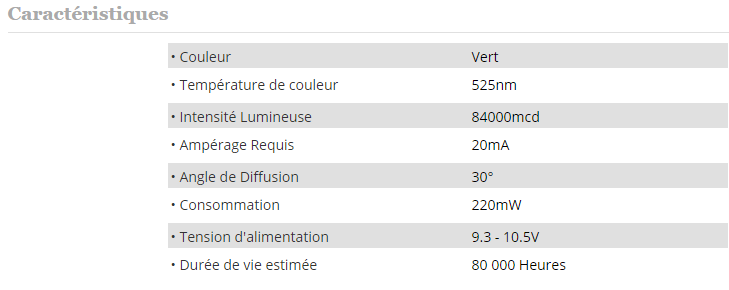
\includegraphics[scale=0.8]{fig/LedDataSheet.png}}
  \caption{LED Datasheet}
  \label{fig:LEDdatasheet}
\end{figure}

\chapter{CCD Properties}
\label{CCDdatasheet}
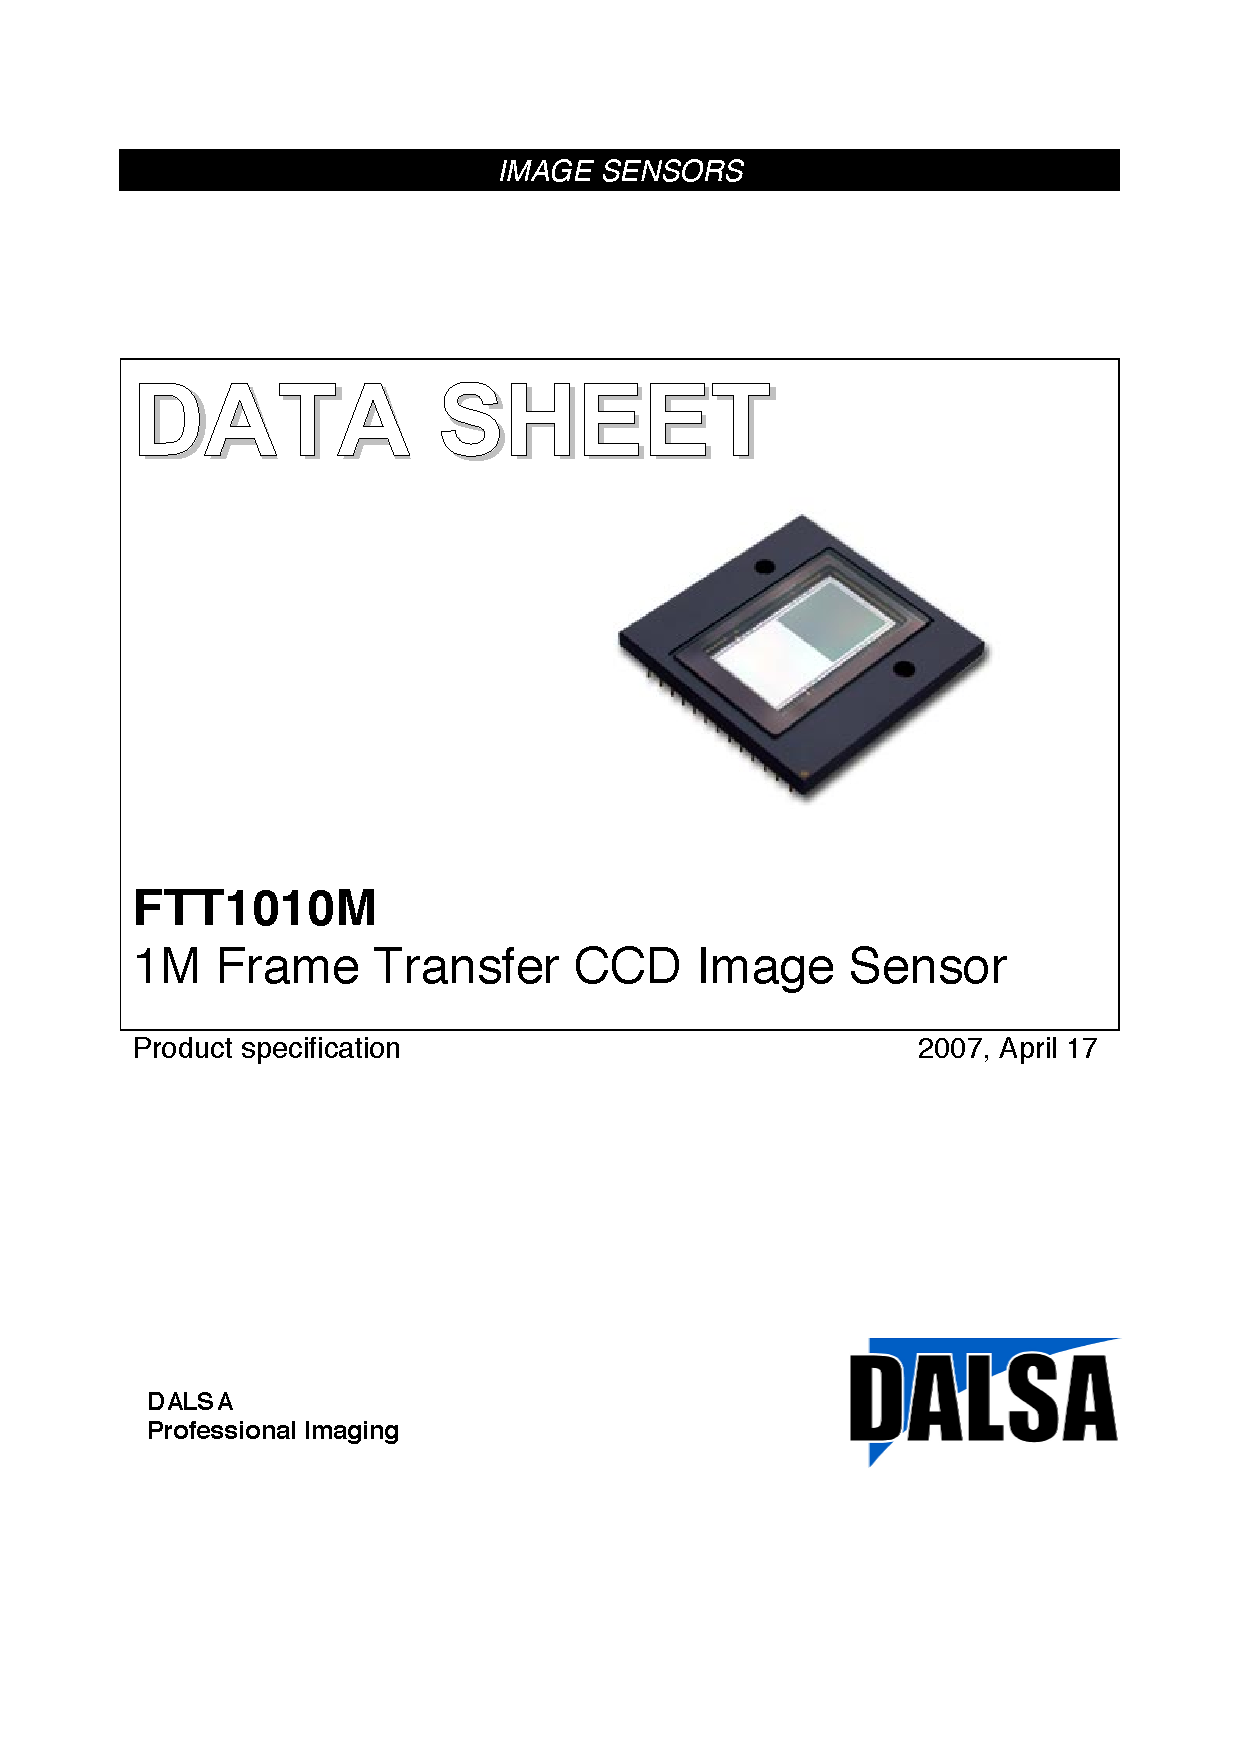
\includepdf[pages = {1-18}]{fig/CCDdatasheet.pdf}

%\end{appendices}

\bibliography{bibliographie}
\bibliographystyle{plain}

\end{document}
